A presente seção tem como propósito estabelecer os fundamentos conceituais, técnicos e científicos que sustentam o desenvolvimento desta pesquisa. Buscando, assim, situar o leitor no contexto interdisciplinar que integra fenômenos físico-mecânicos, técnicas de aquisição e análise de sinais, algoritmos de aprendizado de máquina e implementação em hardware reconfigurável.

Inicialmente, apresenta-se a \textbf{Técnica de Emissão Acústica (EA)} como ferramenta de ensaio não destrutivo, amplamente utilizada para o monitoramento de processos de degradação estrutural e detecção de falhas em sistemas hidráulicos e rotativos. São discutidos o funcionamento, os parâmetros característicos dos sinais e os avanços na aplicação da EA à identificação de cavitação em bombas centrífugas.

Em seguida, aborda-se o \textbf{Aprendizado de Máquina (\textit{Machine Learning, ML})}, com ênfase nas arquiteturas de \textbf{Redes Neurais Convolucionais Unidimensionais (\textit{One-Dimensional Convolutional Neural Network, CNN-1D})}, que têm se destacado no processamento de sinais acústicos e vibracionais. São apresentados os principais paradigmas de aprendizado, os algoritmos mais utilizados na literatura e as bases matemáticas que fundamentam as CNNs aplicadas à análise espectro-temporal de sinais de Emissão Acústica.

Por fim, introduz-se o conceito de \textbf{Field-Programmable Gate Arrays (FPGAs)}, destacando suas características de paralelismo, baixa latência e reconfigurabilidade, que as tornam plataformas ideais para o processamento em tempo real de dados provenientes de sensores inteligentes. Discute-se ainda o potencial de integração entre aprendizado de máquina e hardware reconfigurável, abrindo caminho para \mbox{sistemas embarcados de diagnóstico autônomo.}

Cada uma das seções é acompanhada de uma subseção dedicada à \textit{análise de trabalhos correlatos}, que contextualiza os principais avanços e lacunas na literatura, servindo de base para o delineamento da proposta apresentada nesta dissertação.


\section{Uso de Emissão Acústica na Detecção de Falhas}\label{sec:UsoEA}

Nesta seção, apresenta-se a técnica de Emissão Acústica, EA, como uma ferramenta poderosa de ensaio não destrutivo para o monitoramento e diagnóstico de falhas em sistemas mecânicos e hidráulicos. São discutidos os princípios físicos que regem a geração e propagação das ondas acústicas, os  parâmetros extraídos dos sinais e as etapas envolvidas na aquisição e no tratamento dos dados. Busca-se, ainda, evidenciar a relevância da EA na detecção de fenômenos como trincas, erosão e cavitação, contextualizando sua evolução histórica e suas aplicações em ambientes industriais de alta criticidade.

A Técnica de Emissão Acústica (EA) estabelece-se como um método robusto e dinâmico de ensaio não destrutivo, destinado ao monitoramento e diagnóstico em tempo real de fenômenos como trincas, deslizamentos dislocacionais, delaminações e transições de fase. Esses eventos liberam energia de forma abrupta, gerando ondas elásticas transitórias que se propagam pela estrutura até serem captadas por sensores piezoelétricos — tipicamente fabricados em cerâmica de titanato-zirconato de chumbo (PZT) — os quais convertem o estímulo mecânico em sinais elétricos mensuráveis.  

A Figura~\ref{fig:nde-ed-org-Fig1} apresenta o diagrama funcional de um sistema de Emissão Acústica multicanal, ilustrando a cadeia completa de aquisição de sinais desde os sensores até o armazenamento e exibição dos dados. Cada canal é composto por uma sequência de estágios eletrônicos responsáveis pela detecção, amplificação, filtragem e digitalização dos sinais acústicos gerados durante os eventos de falha.

\begin{figure}[H]
    \centering
    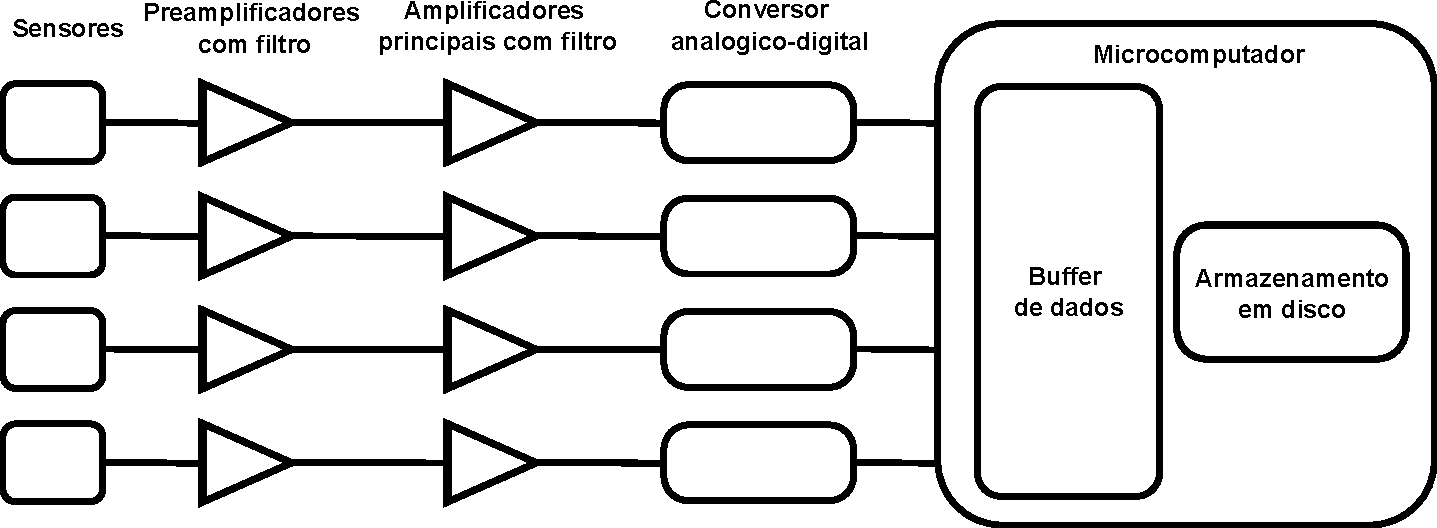
\includegraphics[width=.9\linewidth]{figs/Artigos/nde-ed-org/Figura1.pdf}
    \caption{Esquema funcional de um sistema de Emissão Acústica com sensores piezoelétricos, pré-amplificadores, filtros, amplificadores principais e sistema de aquisição digital. Adaptado de \citeonline{nde-ed-ae-equipment}.}
    \label{fig:nde-ed-org-Fig1}
\end{figure}

Inicialmente, os \textbf{sensores piezoelétricos} são fixados mecanicamente sobre a superfície do corpo de prova ou equipamento monitorado, utilizando acoplantes acústicos para otimizar a transmissão das ondas elásticas. Esses sensores são sensíveis a variações de pressão e deformações locais, produzindo um sinal elétrico \mbox{proporcional à amplitude da onda incidente}.

O sinal gerado pelo sensor é então encaminhado a um \textbf{pré-amplificador}, cuja função é elevar o nível de tensão do sinal original, geralmente na faixa de microvolts, para níveis adequados à posterior amplificação e filtragem. Em muitos sistemas, esse estágio inicial já incorpora filtros passa-faixa (tipicamente entre 100~kHz e 1~MHz), destinados a eliminar componentes de baixa frequência e ruídos ambientais, preservando apenas as frequências características dos eventos acústicos.

Em seguida, o sinal passa por um \textbf{amplificador principal}, também dotado de filtros ajustáveis, que permite o controle do ganho e a supressão de ruídos residuais. Essa dupla amplificação — pré e principal — é essencial para garantir uma relação sinal-ruído satisfatória, sobretudo em medições realizadas em ambientes industriais com \mbox{alta interferência eletromagnética.}

Após o condicionamento analógico, o sinal é direcionado a um \textbf{circuito de medição} que realiza a conversão analógico-digital, ADC, amostrando o sinal em altas taxas (geralmente entre 1~MHz e 40~MHz, dependendo da aplicação e do fenômeno estudado). Esses dados digitalizados são então armazenados temporariamente em um \textbf{\textit{buffer} de dados}, que atua como intermediário entre o \textit{front-end} analógico \mbox{e o sistema de processamento}.

O \textbf{microcomputador} ou unidade de controle central é responsável por gerenciar a aquisição e o armazenamento em disco, além de permitir o processamento dos sinais por meio de algoritmos dedicados à detecção de eventos, cálculo de parâmetros de emissão acústica (como amplitude, duração, energia e contagem de hits) e classificação de padrões. Em sistemas modernos, essa unidade também pode realizar a comunicação com interfaces externas, como APIs industriais, redes MODBUS ou sistemas supervisórios SCADA.

Por fim, o sistema é integrado a módulos de \textbf{visualização e controle}, permitindo que os resultados sejam exibidos em tempo real em um display ou monitor, e que o operador interaja por meio de um teclado ou interface gráfica. Essa visualização pode incluir formas de onda, histogramas de energia, espectros de frequência e alarmes automáticos quando limiares pré-definidos são excedidos.

Em conjunto, os elementos apresentados na Figura~\ref{fig:nde-ed-org-Fig1} compõem um sistema de aquisição e monitoramento de Emissão Acústica capaz de registrar, processar e analisar fenômenos transientes de alta frequência com elevada sensibilidade e precisão temporal. Esse tipo de arquitetura é amplamente empregado em pesquisas e aplicações industriais voltadas à detecção precoce de falhas estruturais, cavitação e fadiga de materiais, oferecendo uma alternativa não invasiva e altamente responsiva aos métodos tradicionais de inspeção.

Após a captação, o sinal adentra um circuito composto por \textbf{pré-amplificador}, \textbf{filtros} e \textbf{amplificador principal}, antes de ser \textbf{digitalizado} para análise computacional. Essa etapa é crucial porque eleva a relação sinal-ruído, atenua interferências eletromagnéticas e rejeita componentes espectrais alheios à banda de interesse; por essa razão, os pré-amplificadores costumam ser posicionados o mais próximo possível da fonte, reduzindo perdas por cabo e mitigando a suscetibilidade a ruídos acoplados.

A análise dos sinais de EA fornece dados cruciais por meio de parâmetros como \textbf{amplitude} (pico do sinal acima do nível de referência), \textbf{tempo de subida} (\textit{rise time}, usualmente do primeiro cruzamento de limiar ao pico), \textbf{duração} (intervalo durante o qual o sinal permanece acima do limiar), \textbf{contagens} (\textit{counts}, número de cruzamentos do limiar por um circuito comparador) e uma medida de \textbf{energia} associada ao evento. Na terminologia do \citeonline{nde-ed-ae-equipment}, essa energia é frequentemente chamada de \textbf{MARSE} (\textit{measured area under the rectified signal envelope}) e corresponde, de forma simplificada, à \textit{área sob o invólucro retificado} do sinal durante a janela do evento; detalhes são esquematizados na Figura~\ref{fig:nde-ed-org-Fig2}. Tais parâmetros não apenas permitem identificar e caracterizar “\textit{hits}” de emissão, mas também se prestam à separação entre ocorrências significativas e ruído de fundo, funcionando como indicadores robustos dos mecanismos físicos subjacentes ao dano.

\begin{figure}[H]
    \centering
    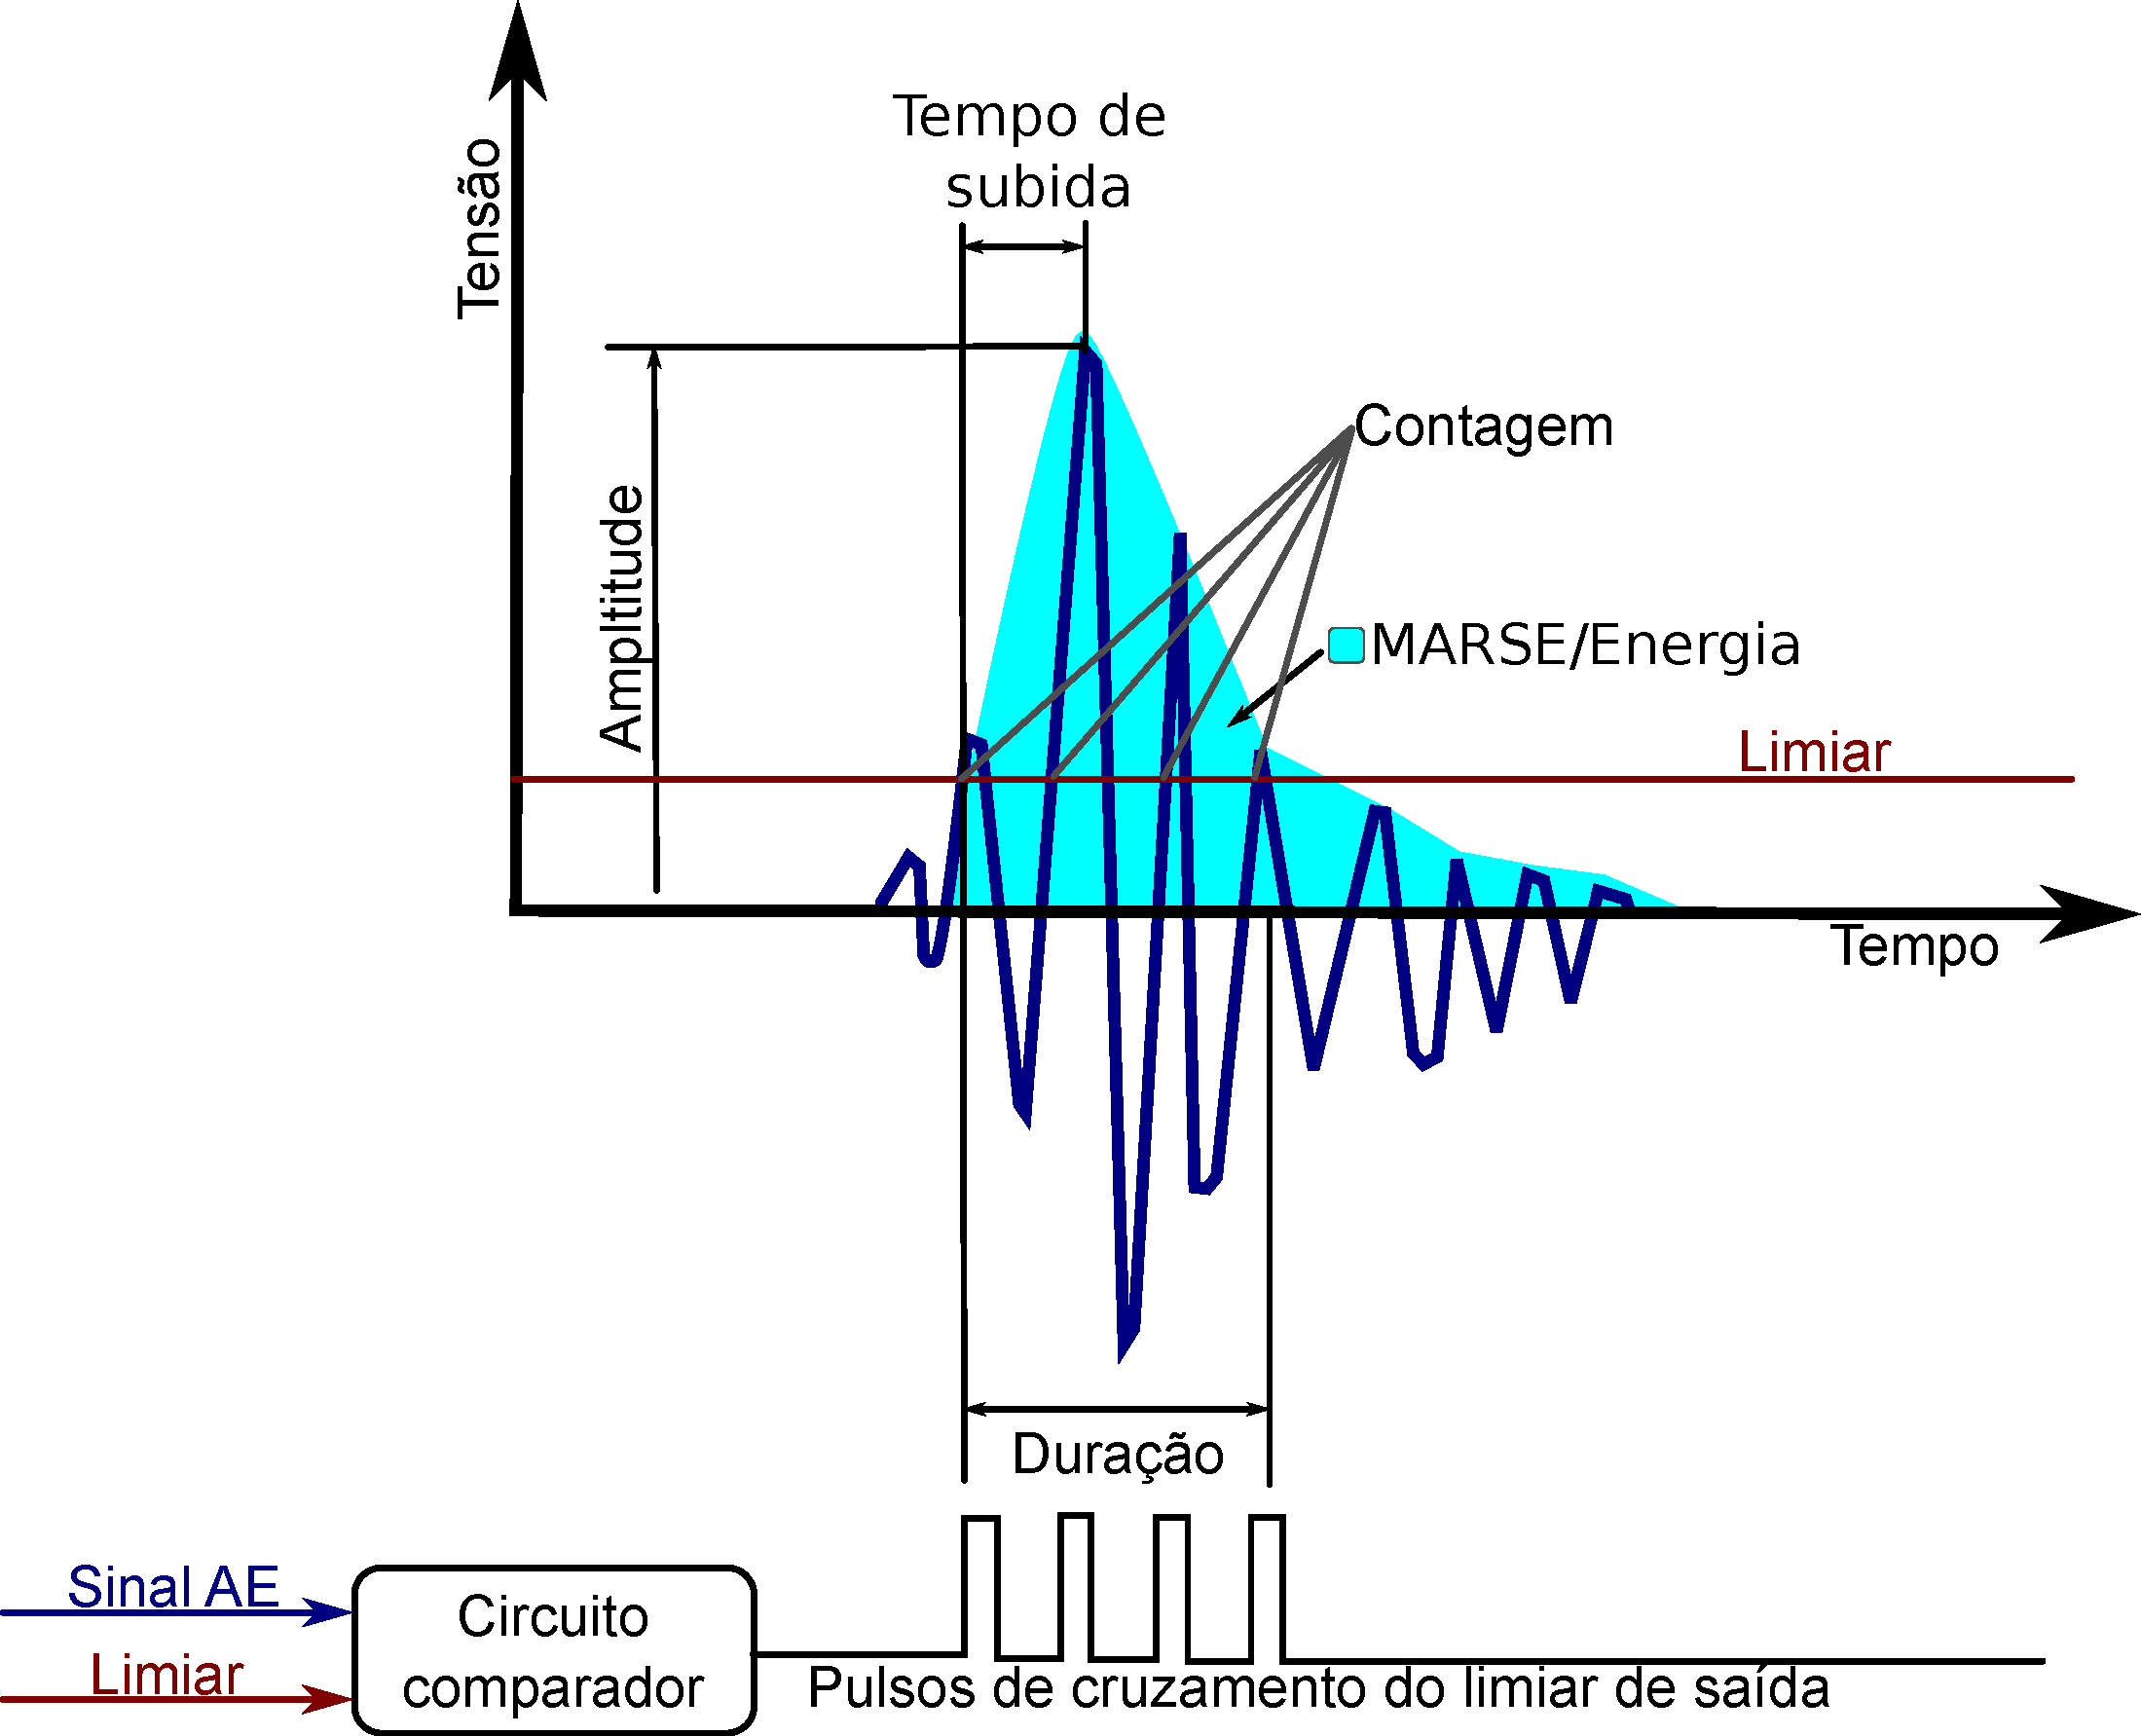
\includegraphics[width=.7\linewidth]{figs/Artigos/nde-ed-org/Figura2.pdf}
    \caption{Parâmetros clássicos extraídos de um “hit” de EA: amplitude, tempo de subida (\textit{rise time}), duração, contagens de limiar (\textit{counts}) e medida de energia (MARSE). O circuito comparador gera pulsos a cada cruzamento do limiar, contabilizados pelo sistema (adaptado de \citeonline{nde-ed-ae-equipment}).}
    \label{fig:nde-ed-org-Fig2}
\end{figure}

Do ponto de vista operacional, o \textbf{limiar} (\textit{threshold}) é definido sobre o nível de ruído para que a detecção seja seletiva. Um \textbf{hit} inicia no primeiro cruzamento desse limiar e se encerra quando o sinal permanece abaixo dele por um tempo de \textit{hit lockout} pré-definido. A partir daí, decompõem-se as grandezas:
\begin{itemize}
    \item \textbf{Amplitude} ($A_\text{pico}$): valor máximo do sinal acima do nível de referência dentro do hit.
    \item \textbf{Tempo de subida} ($t_\text{rise}$): intervalo do primeiro cruzamento de limiar até $A_\text{pico}$; é sensível à cinemática da fonte e à resposta do caminho de propagação.
    \item \textbf{Duração} ($t_\text{dur}$): tempo entre o primeiro e o último cruzamento do limiar; aumenta na presença de reverberações e múltiplas reflexões.
    \item \textbf{Contagens} (\textit{counts}): número de pulsos gerados pelo comparador a cada cruzamento de limiar; correlaciona-se com o conteúdo de alta frequência e a “granulosidade” do evento.
    \item \textbf{Energia (MARSE)}: área sob o invólucro retificado do sinal dentro da janela do hit.Matematicamente, a forma \textit{MARSE} pode ser escrita, em uma discretização simples,~como apresentada em \ref{eq:marse}. 
    
    \begin{equation}
    	\label{eq:marse}
    	\text{MARSE} \;\approx\; \sum_{n=n_0}^{n_1} \big|\,x[n]\,\big| \;\Delta t
    	\quad\text{ou}\quad
    	\text{MARSE} \;\approx\; \sum_{n=n_0}^{n_1} e[n] \;\Delta t,
    \end{equation}
    %$$
    %\text{MARSE} \;\approx\; \sum_{n=n_0}^{n_1} \big|\,x[n]\,\big| \;\Delta t
    %\quad\text{ou}\quad
    %\text{MARSE} \;\approx\; \sum_{n=n_0}^{n_1} e[n] \;\Delta t,
    %$$
    
    em que $x[n]$ é o sinal de EA amostrado e $e[n]$ denota o invólucro (por exemplo, obtido por retificação + filtragem passa-baixas, ou por transformada de Hilbert). Essa métrica captura \textit{quanta de atividade} ao longo do hit, sendo bastante utilizada por fornecedores de instrumentação de EA e por materiais de referência \mbox{educacionais como o \citeonline{nde-ed-ae-equipment}.}
\end{itemize}

\noindent\textbf{{Observação sobre nomenclatura de energia.}}

É importante salientar que \textbf{não há consenso terminológico} na literatura quanto à ``energia'' do evento de EA. Enquanto o \citeonline{nde-ed-ae-equipment} emprega \textit{MARSE} (área do invólucro retificado), revisões de estado da arte, como \citeonline{liu2023review}, frequentemente utilizam \textbf{energia baseada em potência instantânea}, aproximada pela soma dos quadrados da amplitude (proporcional a energia acústica sob hipóteses de linearidade do caminho e calibração adequada, \mbox{como apresentada em \ref{eq:energia}:}

\begin{equation}
	\label{eq:energia}
	E_\text{sq} \;\propto\; \sum_{n=n_0}^{n_1} x^2[n] \;\Delta t.
\end{equation}

Em aplicações comparativas,por exemplo, na distinção entre cavitação incipiente e regimes estabelecidos,essa diferença \textit{conceitual} pode impactar limiares de decisão, escalas de normalização e correlações com grandezas físicas. Por isso, ao longo desta dissertação, quando nos referirmos a \textbf{MARSE}, estaremos explicitamente adotando a \textit{área do invólucro retificado}; quando nos referirmos à \textbf{energia quadrática} (ou simplesmente “energia” na acepção de \citeonline{liu2023review}), estaremos empregando a soma dos quadrados da amplitude. Sempre que pertinente, serão fornecidas ambas as métricas, devidamente normalizadas, de modo a preservar a comparabilidade com diferentes fontes bibliográficas e práticas~de~instrumentação.


O diferencial da técnica reside em seu caráter passivo — ela ``ouve'' a emissão real do material sob carga, ao invés de estimular o componente, como ocorre em métodos como ultrassom ou radiografia. Isso permite monitoramento contínuo e não intrusivo em condições operacionais reais, captando apenas fontes ativas de dano e cobrindo grandes volumes estruturais com um número reduzido de sensores.

Além disso, sistemas de EA podem operar com localização acústica da fonte emissora, utilizando redes de sensores e analisando as diferenças de tempo de chegada do sinal (métodos linear, planar ou volumétrico), o que permite determinar a posição exata de emissão dentro da estrutura.

Esses parâmetros, além de fornecerem informações físicas sobre a natureza do evento, constituem também a base para a extração de \textit{features} no contexto de aprendizado de máquina. Em abordagens modernas de análise de sinais de Emissão Acústica, como a proposta neste trabalho, o conjunto de atributos derivados desses parâmetros — tanto no domínio do tempo quanto no domínio da frequência — é utilizado para representar cada evento (\textit{hit}) de forma compacta e informativa, facilitando sua posterior~classificação~por~redes neurais.

No domínio do tempo, são extraídos descritores diretos, como amplitude, duração, tempo de subida, energia (MARSE ou energia quadrática), número de contagens e razão entre parâmetros (por exemplo, a razão entre energia e duração, indicativa da intensidade relativa do evento). Já no domínio da frequência, técnicas de análise espectral, como a Transformada Rápida de Fourier (FFT) ou a Transformada de Short-Time Fourier (STFT), permitem a identificação de componentes dominantes e a distinção entre regimes acústicos característicos — como cavitação incipiente, cavitação plena e ruído mecânico.

Durante o pré-processamento, esses parâmetros são normalizados com base em janelas móveis e limiares de ruído, garantindo que variações instrumentais ou ambientais não influenciem indevidamente o processo de aprendizagem. As janelas de tempo são segmentadas e rotuladas conforme as classes de operação (\textit{normal}, \textit{cavitação} ou \textit{falha estrutural}), e o conjunto de sinais normalizados é então utilizado como \mbox{entrada para o treinamento da CNN-1D.}

Nesse contexto, a rede convolucional atua como uma extensão automática do processo de extração de \textit{features}, aprendendo representações hierárquicas diretamente das formas de onda ou dos espectrogramas derivados. Essa combinação entre parâmetros clássicos da Emissão Acústica e aprendizado profundo forma uma abordagem híbrida que alia a interpretabilidade dos métodos tradicionais à robustez e adaptabilidade dos modelos modernos de Inteligência Artificial, conforme ilustrado no fluxograma geral dos objetivos~da pesquisa (Figura~\ref{fig:fluxograma_geral}).

Ademais, a onda primitiva originada em um evento de EA é tipicamente de curta duração (microssegundos) e pode apresentar forte direcionalidade e variabilidade na amplitude, dependendo da natureza física da falha, como deformação cristalina ou fraturas progressivas. Sua propagação é influenciada por fatores como atenuações geométricas, estruturais e pela dispersão devido à microestrutura do material, \mbox{como os contornos de grão e inclusões.}

É importante ressaltar que nem toda emissão EA indica falha estrutural: fenômenos como fricção mecânica, vazamentos e pulsos por cavitação ou descargas parciais podem produzir sinais semelhantes aos genuínos, classificados como pseudo-fontes. A aplicação de filtros avançados, avaliação espectral e critérios baseados em tempo de chegada são estratégias fundamentais para distinguir esses eventos e minimizar falsos positivos.

Em síntese, a técnica de Emissão Acústica apresenta-se como uma abordagem promissora para o monitoramento em tempo real e a detecção precoce de falhas estruturais, devido à sua alta sensibilidade e natureza não intrusiva. A compreensão de seus princípios físicos e dos parâmetros característicos extraídos dos sinais é essencial para a correta interpretação dos fenômenos observados, como trincas, desgaste superficial e cavitação em bombas centrífugas. A seguir, são discutidos estudos representativos que exploram a aplicação da Emissão Acústica em sistemas hidráulicos e turbomáquinas, evidenciando as metodologias empregadas, os resultados obtidos e as limitações que \mbox{motivam o presente~trabalho.}

\subsection{Revisão de Pesquisas sobre Emissão Acústica}

Segundo \citeonline{liu2023review}, a cavitação em bombas é um fenômeno multifásico inevitável que provoca a formação e colapso de bolhas quando a pressão local do escoamento cai abaixo da pressão de vapor do líquido. Esse processo resulta em perda de desempenho hidráulico, erosão de componentes, vibração excessiva e ruído característico, podendo até gerar falhas estruturais. A detecção precoce, portanto, tem grande relevância tanto para a segurança operacional quanto para a redução de custos de manutenção.

Os autores revisam diferentes metodologias de detecção baseadas em sinais, como vibração, emissão acústica, ruído hidrodinâmico e pulsação de pressão. Conforme ilustrado no fluxograma da Figura~\ref{fig:LiuFig1}, tais métodos seguem um fluxo comum: aquisição de sinais em pontos estratégicos da bomba, processamento nos domínios do tempo, frequência ou tempo–frequência, extração de parâmetros característicos e, por fim, identificação do estado de cavitação com auxílio de algoritmos de inteligência artificial. A Figura~\ref{fig:LiuFig2} resume essas metodologias de pesquisa.

\begin{figure}[H]
    \centering
    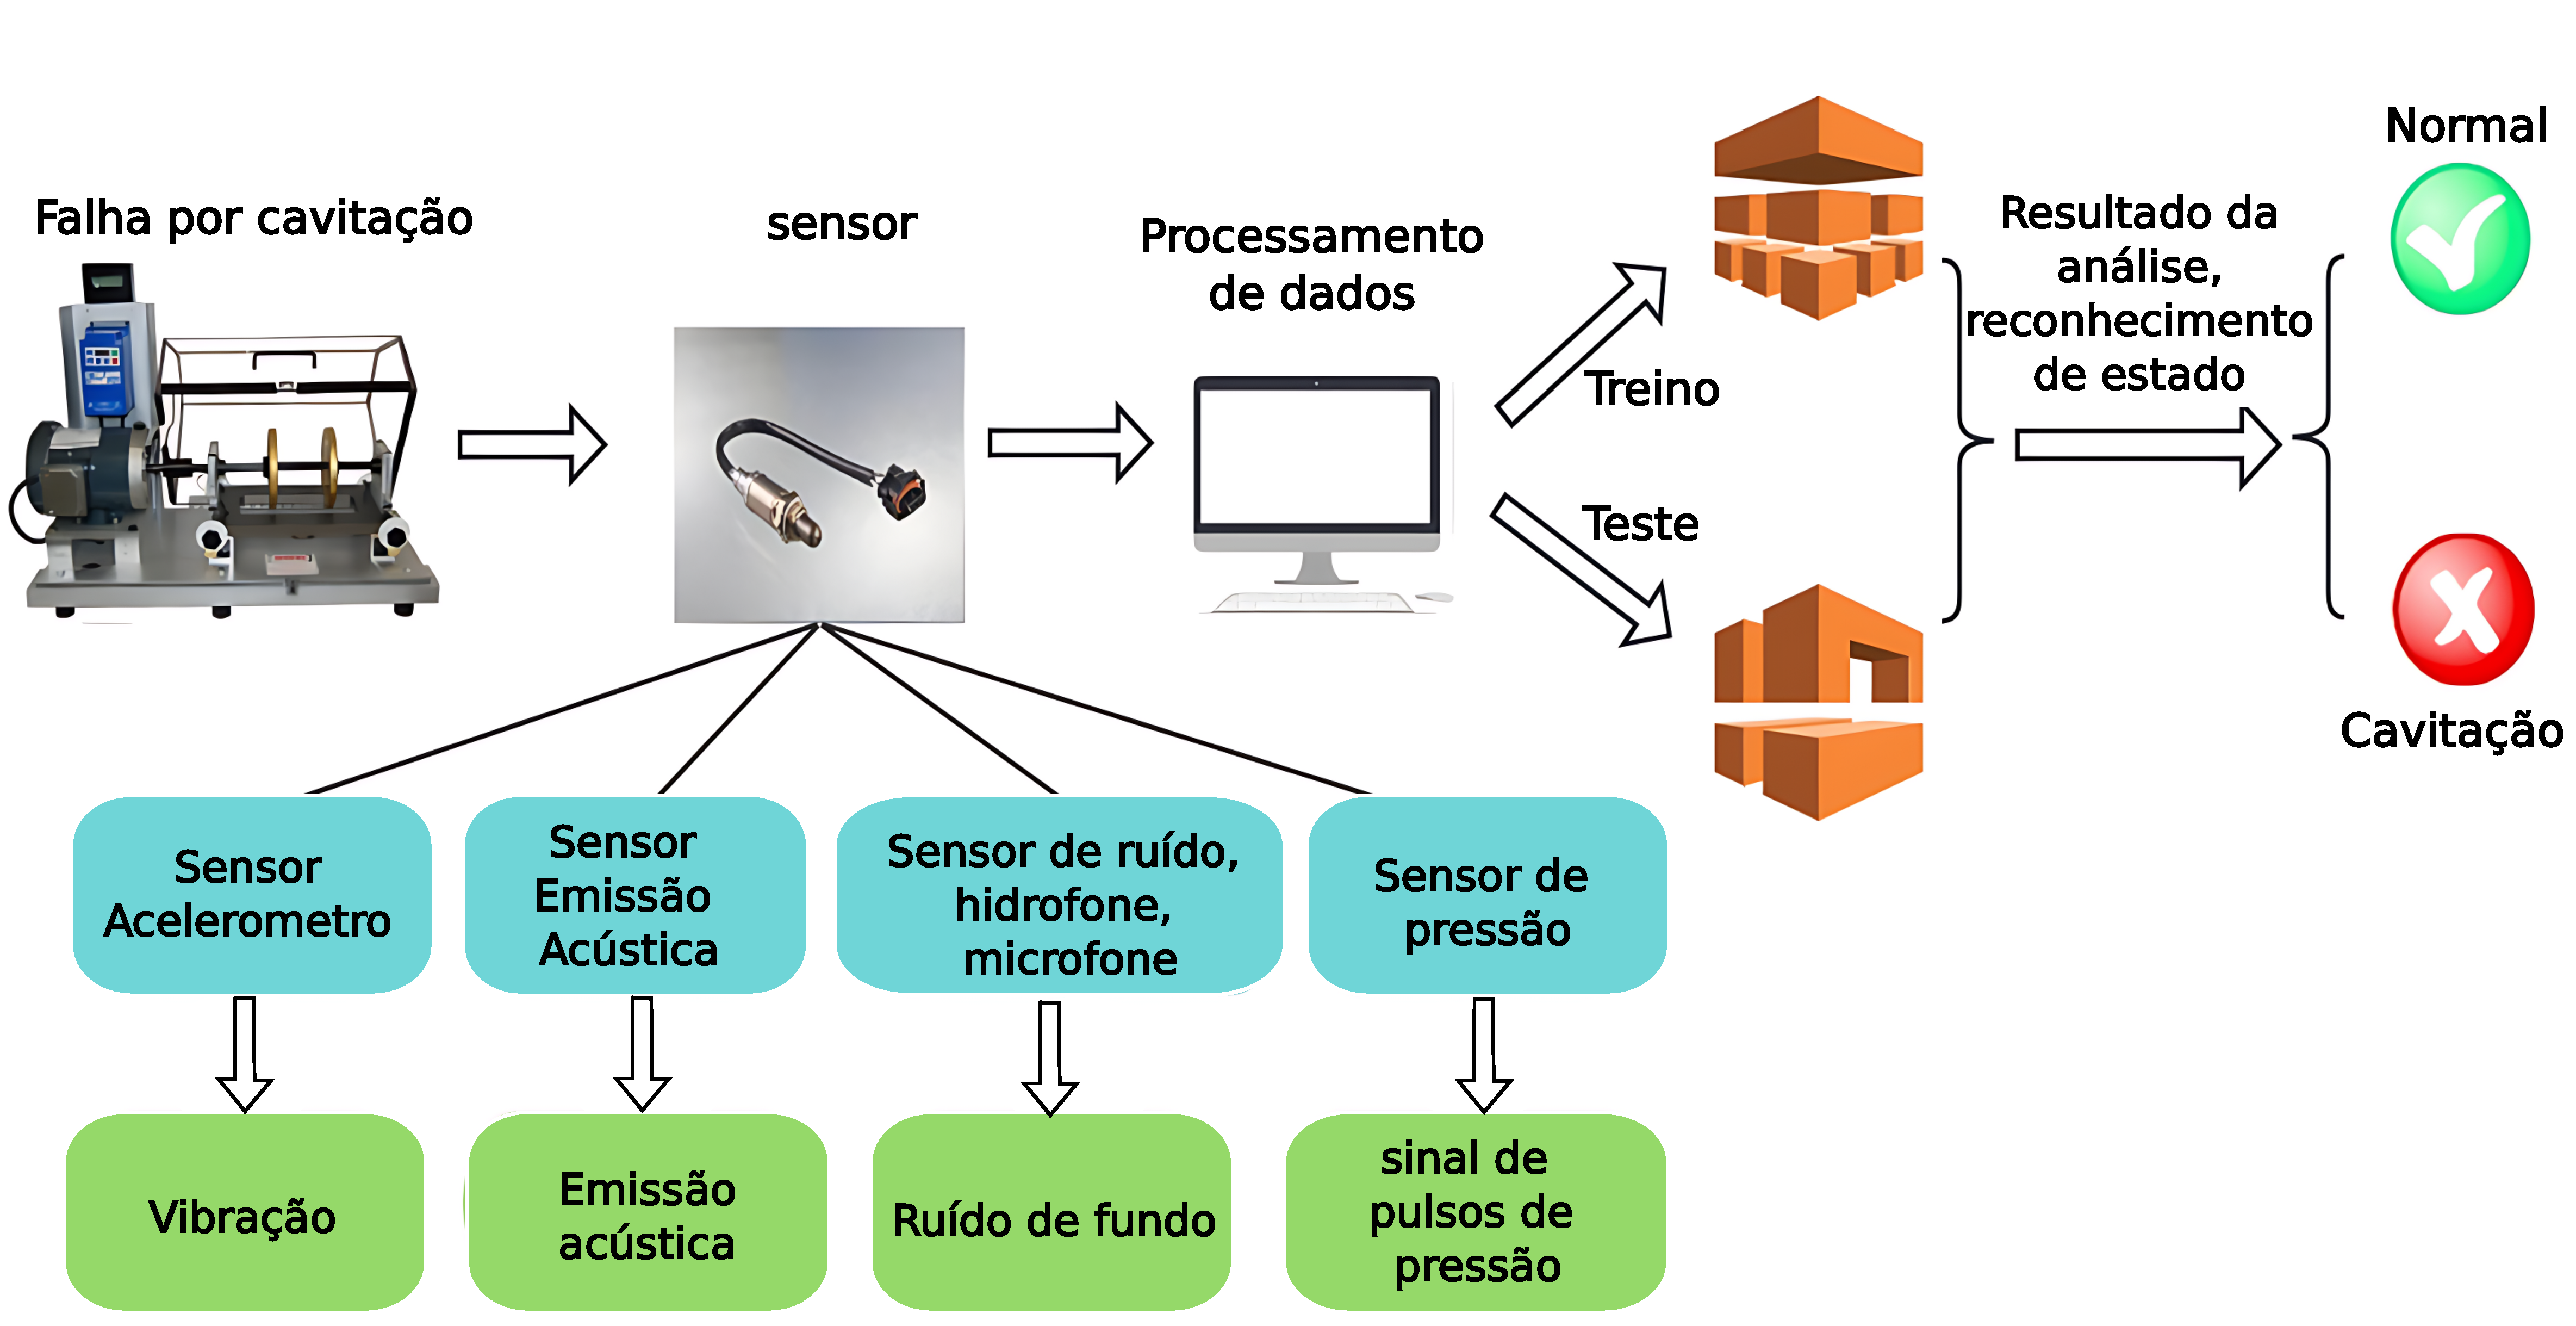
\includegraphics[width=1\linewidth]{figs/Artigos/Liu/Figura1.pdf}
    \caption{Fluxograma básico de detecção de cavitação com base em diferentes sinais. Adaptado de \citeonline{liu2023review}.}
    \label{fig:LiuFig1}
\end{figure}

O diagrama da Figura~\ref{fig:LiuFig1} organiza a detecção por \textbf{famílias de sinais} e explicita a relação entre a física da cavitação e o canal sensorial:
\begin{itemize}
    \item \textbf{Sinal de vibração (acelerômetros):} sensível à excitação mecânica do conjunto rotor–estator; captura impactos e modulações de banda larga provocadas pelo colapso de bolhas e por fenômenos associados, entre outros efeitos (desbalanceamento secundário, instabilidades hidráulicas).
    
    \item \textbf{Sinal de emissão acústica (sensores piezoelétricos):} focaliza faixas de alta frequência (tipicamente centenas de kHz), nas quais eventos transientes de cavitação apresentam razão sinal–ruído elevada; adequado à detecção incipiente.
    \item \textbf{Sinal de ruído (microfones/hidrofones):} capta componentes aéreas ou no fluido; informativo para estágios mais intensos de cavitação e para varreduras rápidas, embora mais suscetível a interferências ambientais.
    \item \textbf{Pulsação de pressão (transdutores de pressão):} evidencia flutuações periódicas/quasi-periódicas do campo de pressão; útil para mapear regimes e instabilidades do escoamento.
\end{itemize}
A linha intermediária do diagrama explicita que \textbf{cada sensor observa um aspecto da cavitação}: os sinais carregam assinaturas distintas (impactos, bandas espectrais, intermitência, modulações). A partir daí, o fluxo converge para \textbf{processamento de sinais} (métricas no tempo: RMS, pico, curtose, crest factor; no espectro: centroides, bandas energéticas; no tempo–frequência: STFT, wavelets), seguido de \textbf{extração de atributos} e \textbf{reconhecimento de estado} por algoritmos de IA (por exemplo, \textit{SVM}, \textit{Random Forest}, \textit{k-NN}, e redes profundas como CNN-1D/2D ou \textit{LSTM}). Em síntese, a figura mostra que, embora os canais sensoriais sejam diversos, o \textit{pipeline lógico} é comum e modular.

\begin{figure}[H]
    \centering
    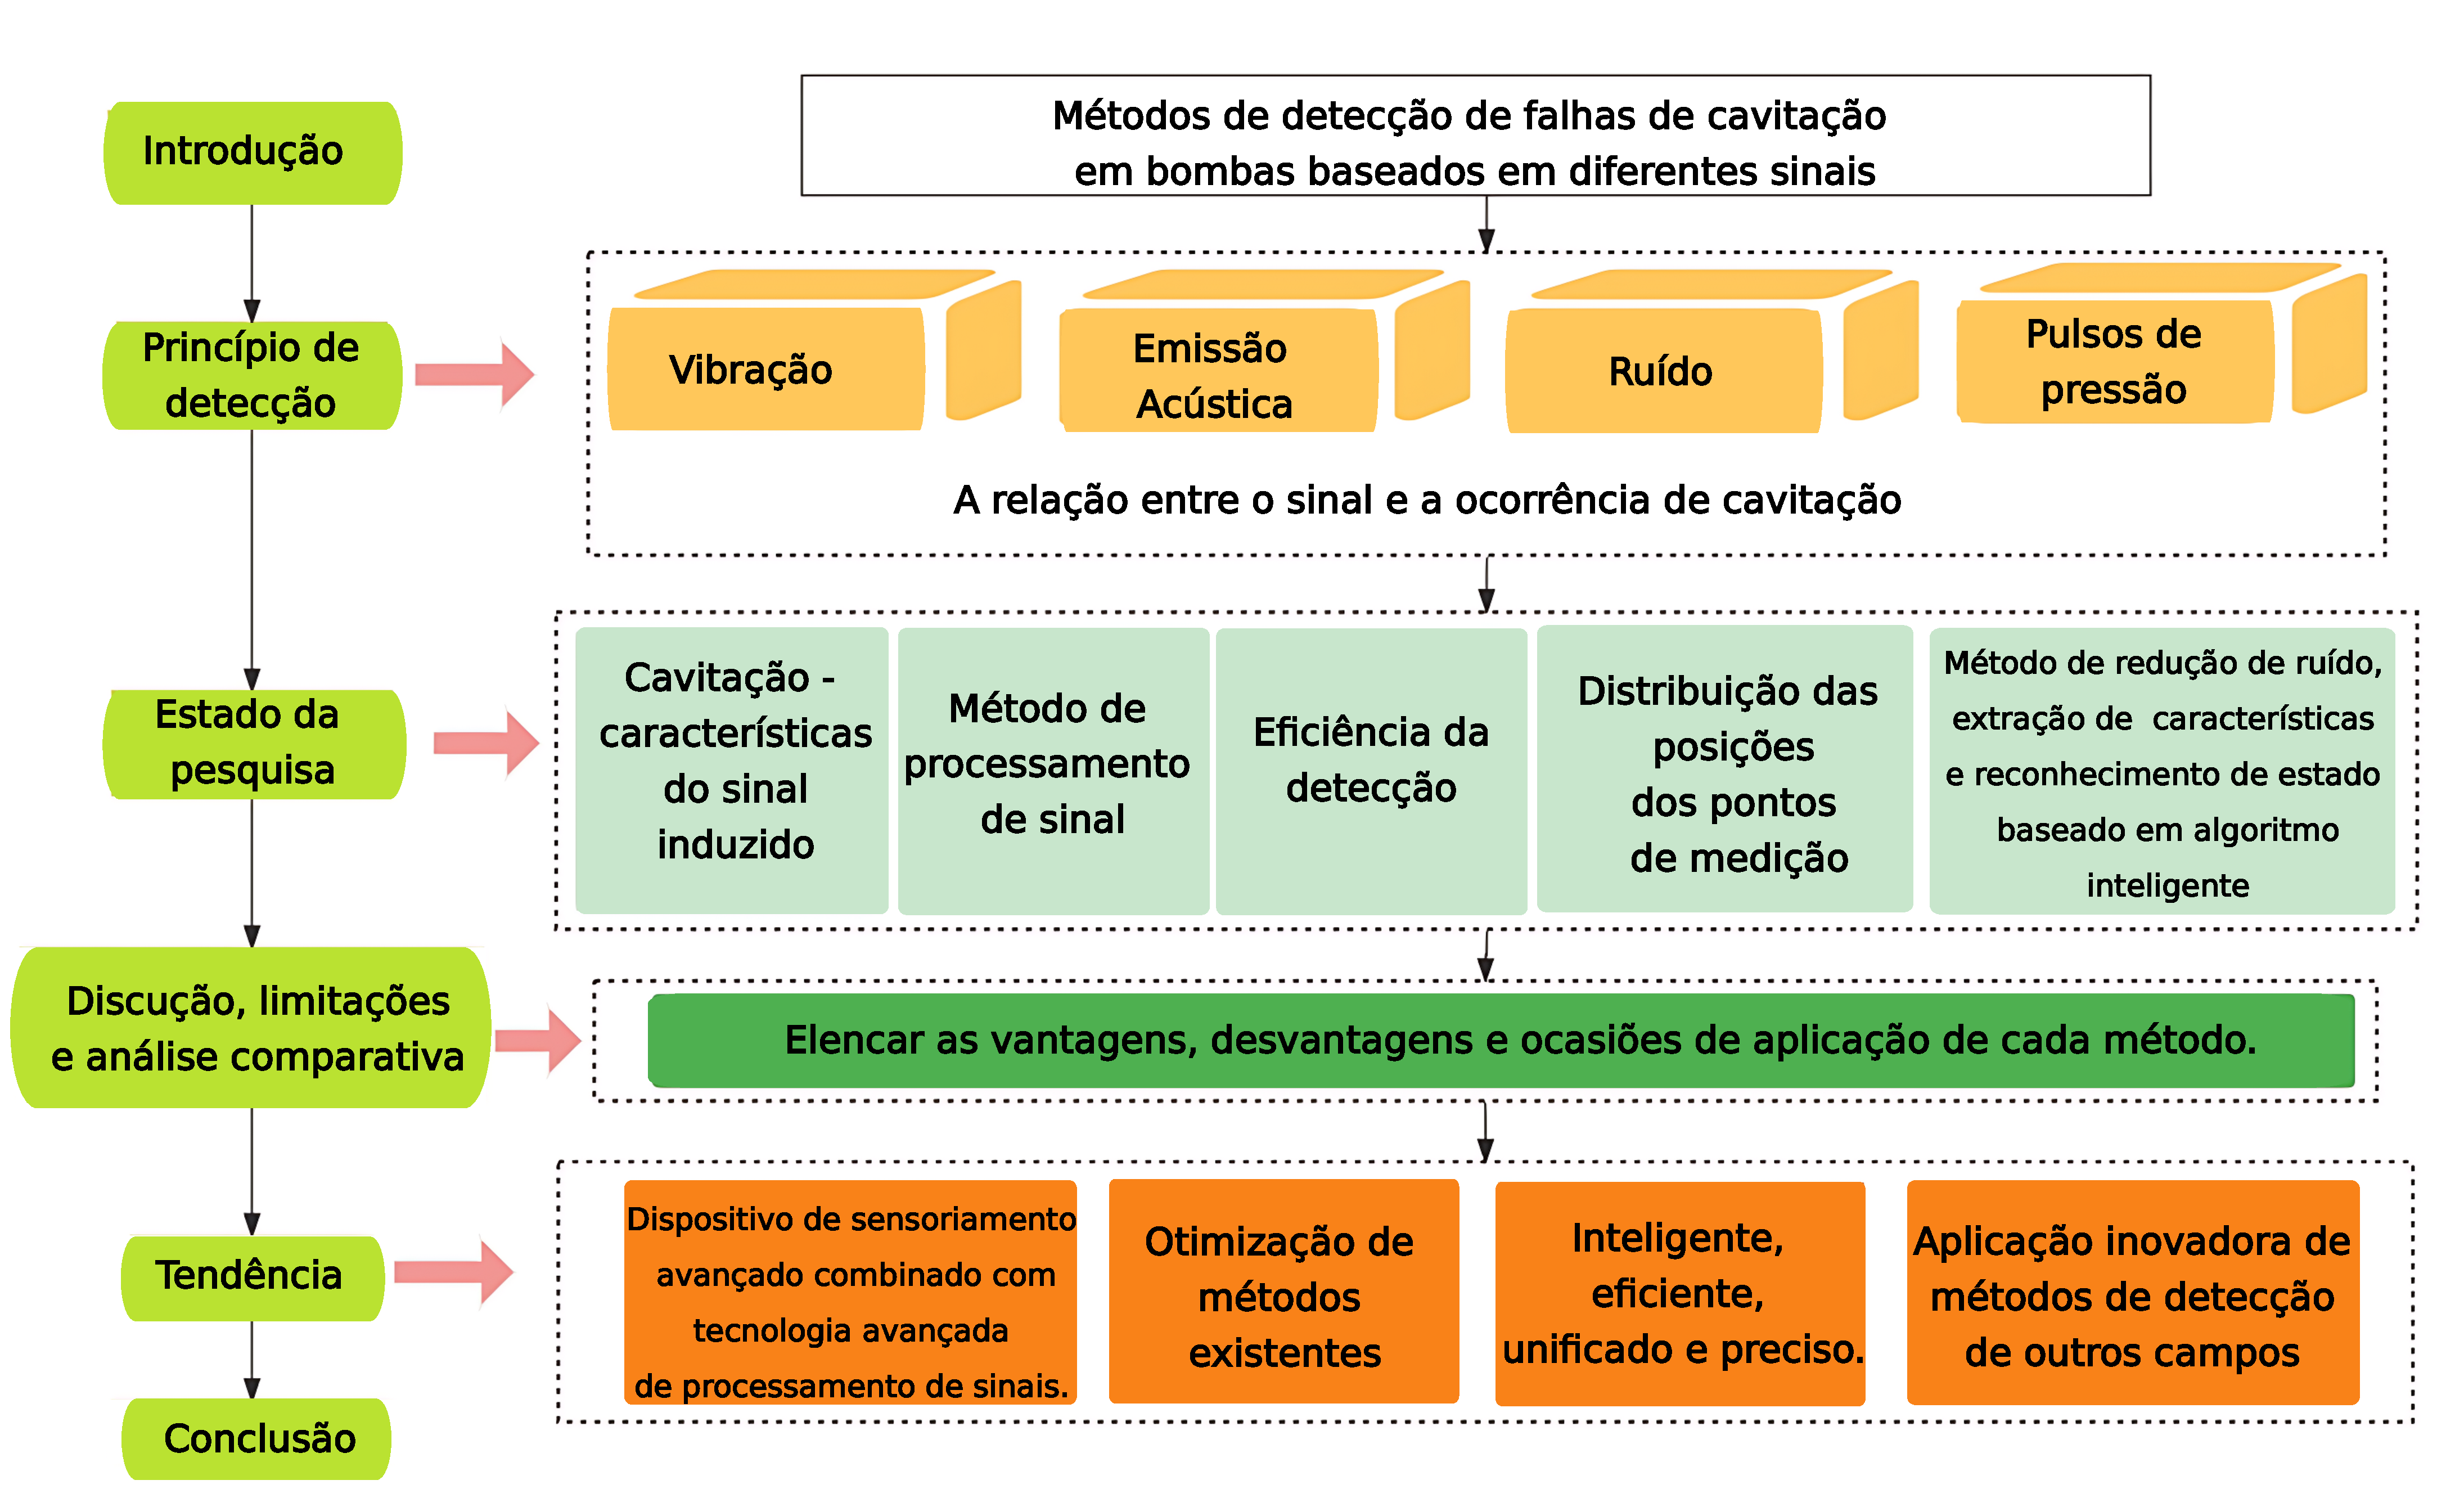
\includegraphics[width=1\linewidth]{figs/Artigos/Liu/Figura2.pdf}
    \caption{Diagrama principal do conteúdo da pesquisa do artigo. Adaptado de \citeonline{liu2023review}. }
    \label{fig:LiuFig2}
\end{figure}

Com o objetivo de mapear os desafios do monitoramento de condição, o esquema ilustrado na Figura~\ref{fig:LiuFig2} sintetiza o \textbf{ciclo de pesquisa} em cinco camadas essenciais. Tal segmentação abrange desde a caracterização do problema de desempenho e integridade em bombas até a implementação de soluções inteligentes unificadas, compreendendo os seguintes tópicos:

\linespread{1.27}\selectfont
\begin{enumerate}
    \item \textbf{Introdução:} contextualiza a cavitação como problema de desempenho e integridade; define objetivos (detecção incipiente, redução de custos, aumento de confiabilidade).
    \item \textbf{Princípio de detecção:} relaciona a \textit{origem física} da cavitação com o \textit{que cada sensor enxerga}. Por exemplo, o colapso de bolhas gera altas frequências (AE), enquanto flutuações de pressão se refletem mais nos transdutores de pressão e na vibração de baixa/média frequência.
    \item \textbf{Estado da pesquisa:} quatro eixos críticos:
    \begin{enumerate}[label=\alph*)]
        \item \textit{Características induzidas pela cavitação:} intermitência, assimetria estatística, picos espectrais e alargamento de banda; mudanças em curtose, entropias e taxas de cruzamento por limiar.
        \item \textit{Métodos de processamento de sinais:} do básico (filtros, estatísticas de ordem superior) ao avançado (STFT, CWT, espectrogramas, \textit{scalograms}, cepstra).
        \item \textit{Eficiência de detecção:} métricas (acurácia, sensibilidade, especificidade, AUC, F1), além de latência e robustez a ruído; aqui entram comparações sistemáticas entre algoritmos e sensores.
        \item \textit{Posicionamento de pontos de medição:} trade-offs entre proximidade do fenômeno, acessibilidade, segurança, custo e suscetibilidade a ruído estrutural/ambiental.
    \end{enumerate}
    \item \textbf{Discussão, limitações e comparação:} consolida \textit{vantagens e desvantagens} de cada canal/sensor: AE destaca-se na detecção incipiente e em altas frequências, vibração é amplamente disponível e barata, pressão é direta para regimes hidráulicos, ruído é fácil de instrumentar porém sensível a ambiente. Também discute limitações (calibração, variabilidade do escoamento, repetibilidade, datasets pequenos).
    \item \textbf{Tendências:} quatro direções estratégicas:
    \begin{enumerate}[label=\alph*)]
        \item \textit{Sensoriamento avançado + processamento avançado:} sensores banda-larga, arrays, sincronização multicanal; pipelines tempo–frequência e fusão multimodal.
        \item \textit{Otimização de métodos existentes:} melhor seleção de \textit{features}, redução de dimensionalidade, aprendizado semi-supervisionado e \textit{few-shot}.
        \item \textit{Sistemas inteligentes, unificados e acurados:} do laboratório ao campo, com atenção à \textbf{latência}, \textbf{robustez a ruído} e \textbf{generalização} entre bombas/condições.
        \item \textit{Transferência de métodos de outras áreas:} técnicas maduras de diagnóstico de máquinas, sonar/ultrassom e visão computacional (ex., CNNs 1D/2D, transformers específicos para séries temporais).
    \end{enumerate}
\end{enumerate}


Em síntese, as Figuras \ref{fig:LiuFig1} e \ref{fig:LiuFig2} evidenciam que a detecção de cavitação tem evoluído de abordagens puramente empíricas para arquiteturas \textbf{modulares e orientadas a dados}, nas quais a escolha do sensor, a estratégia de processamento e o modelo de classificação integram-se em um \textit{pipeline} unificado e flexível. Essa estrutura permite adaptar metodologias de diagnóstico a distintos contextos industriais, conciliando precisão, \mbox{tempo de resposta e viabilidade de implementação.}

Sob essa perspectiva, os estudos analisados reforçam a motivação central desta pesquisa: investigar a cadeia de processamento que envolve o \textbf{pré-processamento}, a \textbf{extração e representação de atributos} e a \textbf{classificação por meio de uma CNN-1D}, com o objetivo de alcançar uma detecção de cavitação rápida, robusta e energeticamente eficiente. Ao mesmo tempo, mantém-se a perspectiva de integração futura dessas técnicas em \textit{hardware} reconfigurável, consolidando um caminho viável para soluções embarcadas de monitoramento inteligente.


Entre os diversos métodos analisados por \citeonline{liu2023review}, o monitoramento por vibração se destaca como o mais consolidado e amplamente aplicado em sistemas hidráulicos industriais. Alterações expressivas na resposta espectral, especialmente o surgimento de picos em faixas de 2 kHz a 8 kHz, constituem indicadores diretos da presença de cavitação — fenômeno ilustrado nas Figuras \ref{fig:LiuFig4A} e \ref{fig:LiuFig4B}. A primeira demonstra a diferença temporal entre regimes de operação com e sem cavitação, evidenciando o aumento abrupto da amplitude e da irregularidade do sinal. Já a segunda mostra, no domínio da frequência, o deslocamento da energia espectral e a intensificação de componentes harmônicas conforme a rotação da bomba aumenta, comportamento que reflete a instabilidade hidrodinâmica \mbox{provocada pelo colapso das bolhas.}

Apesar de sua maturidade tecnológica, o método de vibração apresenta sensibilidade limitada à cavitação incipiente, uma vez que os sinais gerados nos estágios iniciais do fenômeno são de baixa amplitude e facilmente mascarados por ruídos mecânicos ou estruturais. Nesse contexto, a técnica de \textbf{Emissão Acústica, EA} desponta como alternativa mais sensível e informativa. Essa abordagem capta as ondas elásticas transitórias geradas por microjatos e choques associados ao colapso de cavidades, abrangendo uma faixa espectral que se estende de aproximadamente 1 kHz a 1 MHz.

Os parâmetros derivados do sinal, como \textbf{amplitude}, \textbf{duração}, \textbf{energia} e \textbf{contagens acima do limiar} (ou “counts”), mostrados na Figura \ref{fig:LiuFig6}, constituem indicadores diretos da intensidade e da frequência de ocorrência dos eventos acústicos. Esses parâmetros — amplamente empregados em sistemas de monitoramento baseados em hits — permitem não apenas detectar a cavitação incipiente, mas também avaliar a severidade do processo de erosão associada. No entanto, sua adoção em ambientes industriais ainda é desafiada por fatores como o custo dos sensores piezoelétricos de alta sensibilidade, a necessidade de acoplamento preciso e a suscetibilidade à interferência estrutural.

Assim, enquanto os sensores de vibração oferecem uma visão global e robusta do comportamento dinâmico do conjunto rotativo, a emissão acústica fornece uma janela privilegiada para o diagnóstico precoce, sendo particularmente promissora para integração futura com plataformas embarcadas de detecção inteligente — foco desta pesquisa.
\linespread{1.25}\selectfont

\begin{figure}[H]
    \centering
    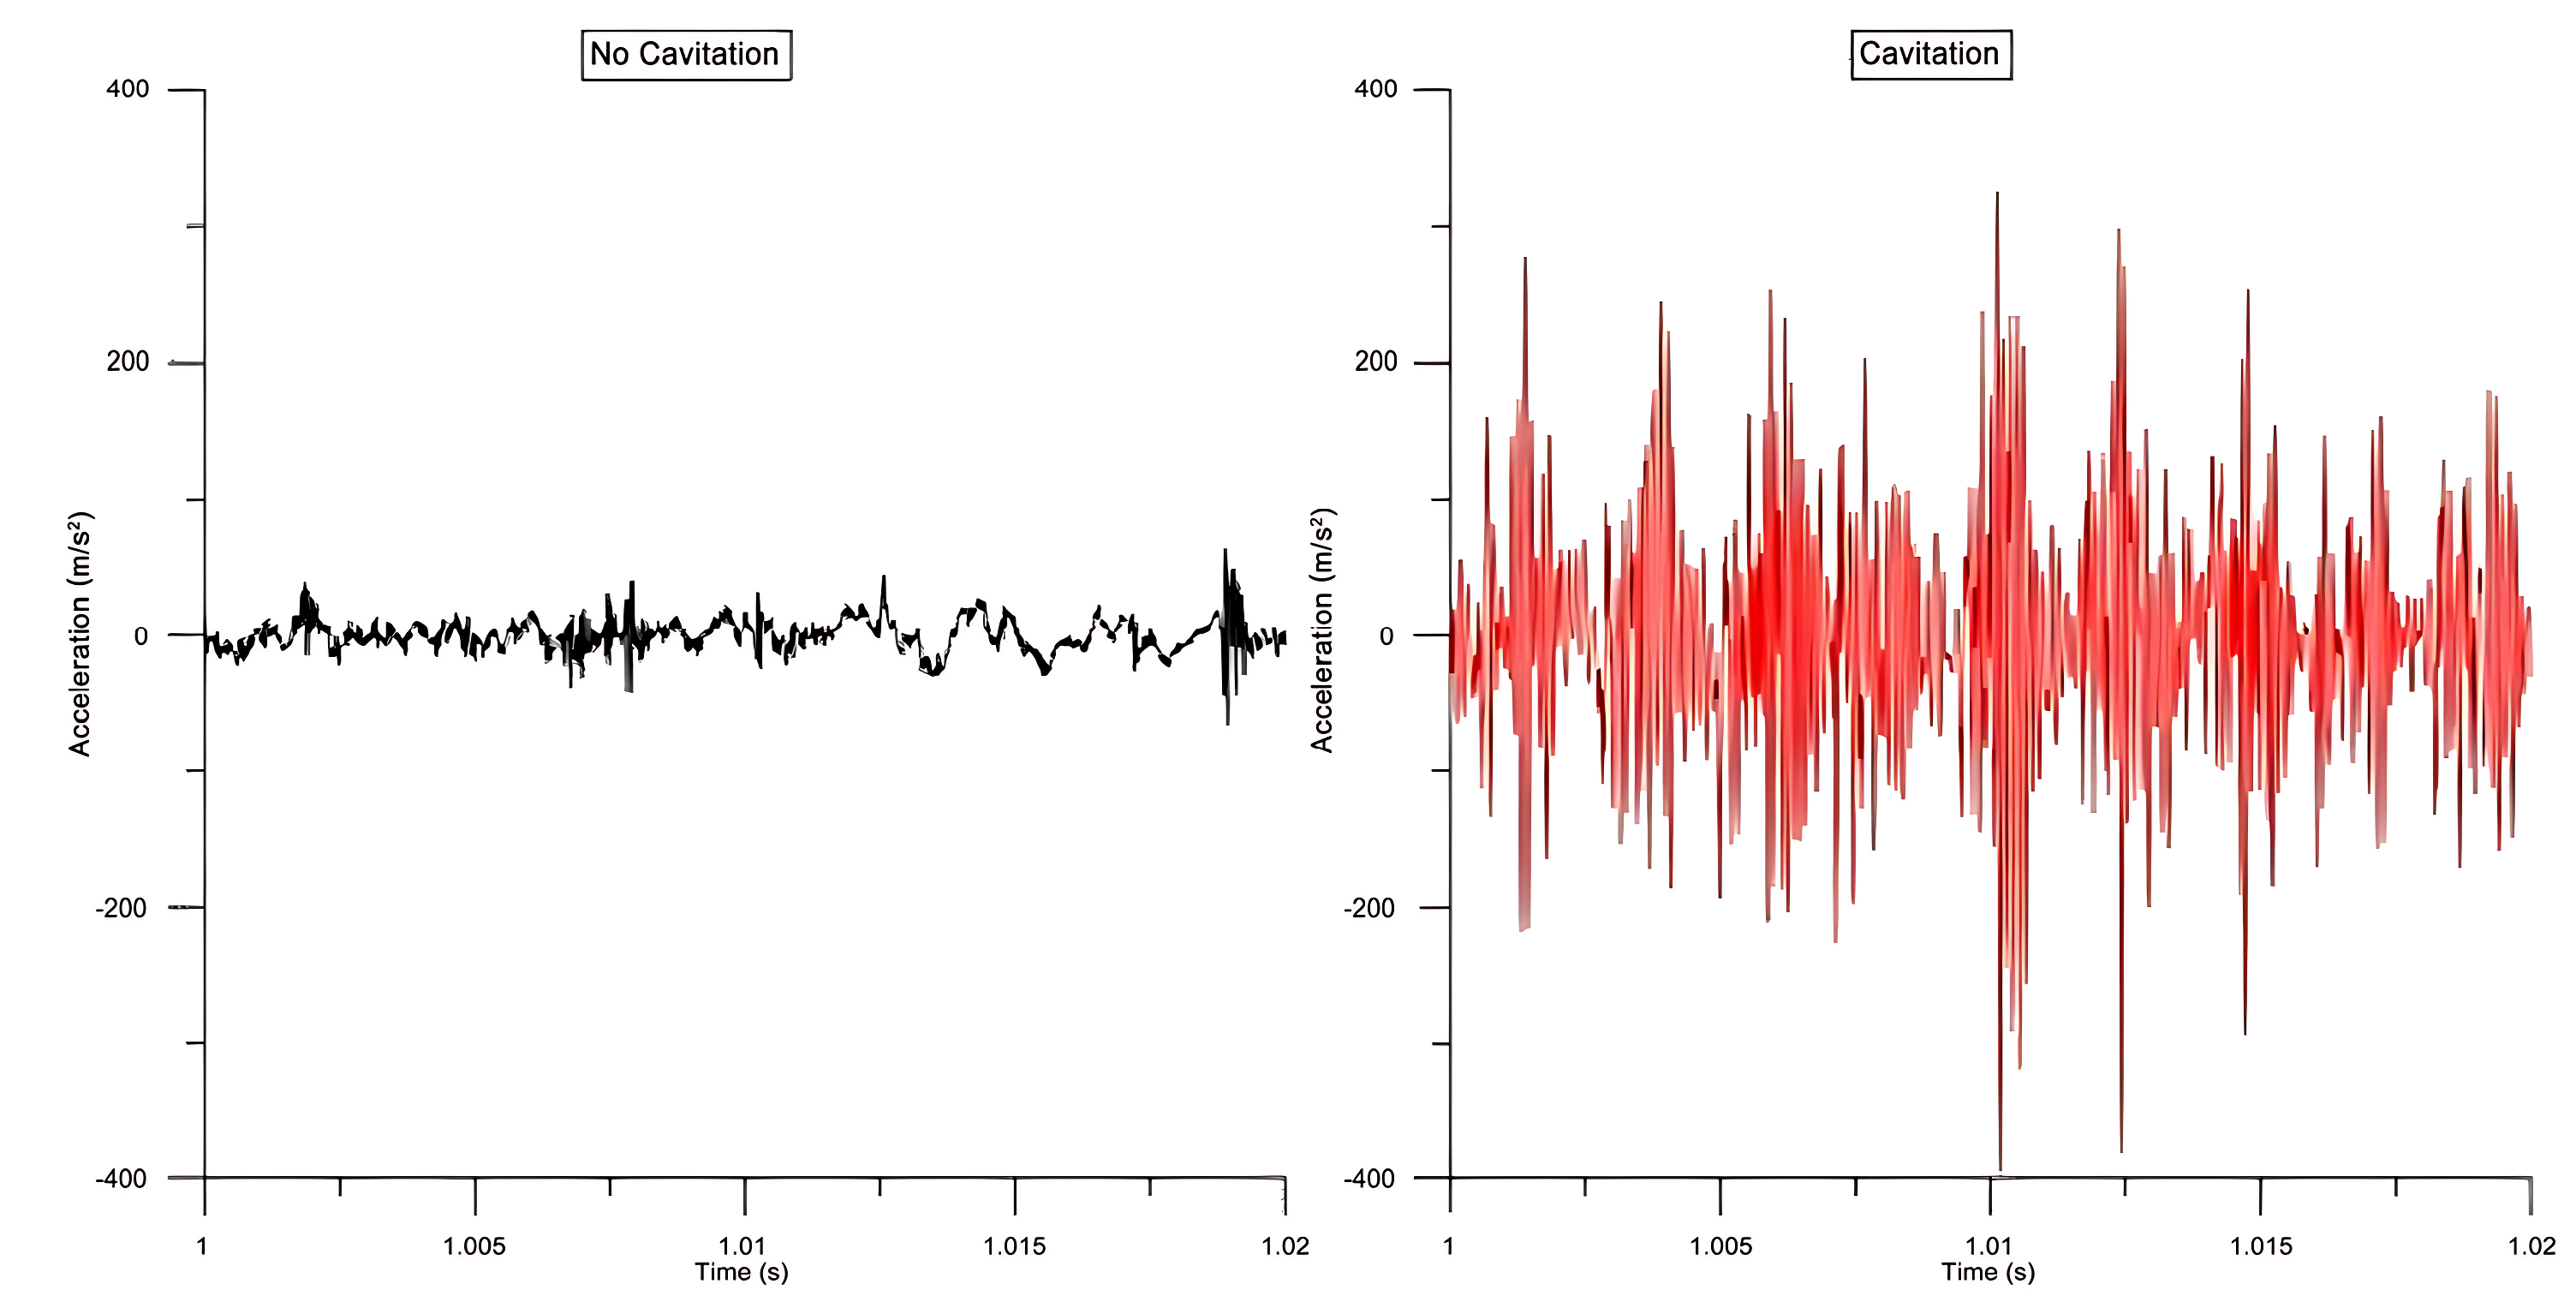
\includegraphics[width=0.95\linewidth]{figs//Artigos//Liu/Figura4A_Upscaler_2K.png}
    \caption{Sinais de aceleração no domínio do tempo em estados de cavitação e não cavitação. Fonte: \citeonline{liu2023review}}
    \label{fig:LiuFig4A}
\end{figure}

A Figura \ref{fig:LiuFig4A} apresenta os sinais de aceleração medidos em uma bomba centrífuga em duas condições distintas: à esquerda, operação normal (sem cavitação), e à direita, sob cavitação. Observa-se que o regime sem cavitação exibe um sinal estável, de baixa amplitude e com pequenas variações associadas ao ruído de fundo e às vibrações naturais da máquina. Em contrapartida, o regime cavitante demonstra um aumento expressivo na amplitude e na irregularidade temporal do sinal, reflexo direto do colapso das bolhas de vapor dentro do fluido. Esse comportamento errático é característico da cavitação e se intensifica com o aumento da velocidade de rotação e da severidade do fenômeno.

\begin{figure}[H]
    \centering
    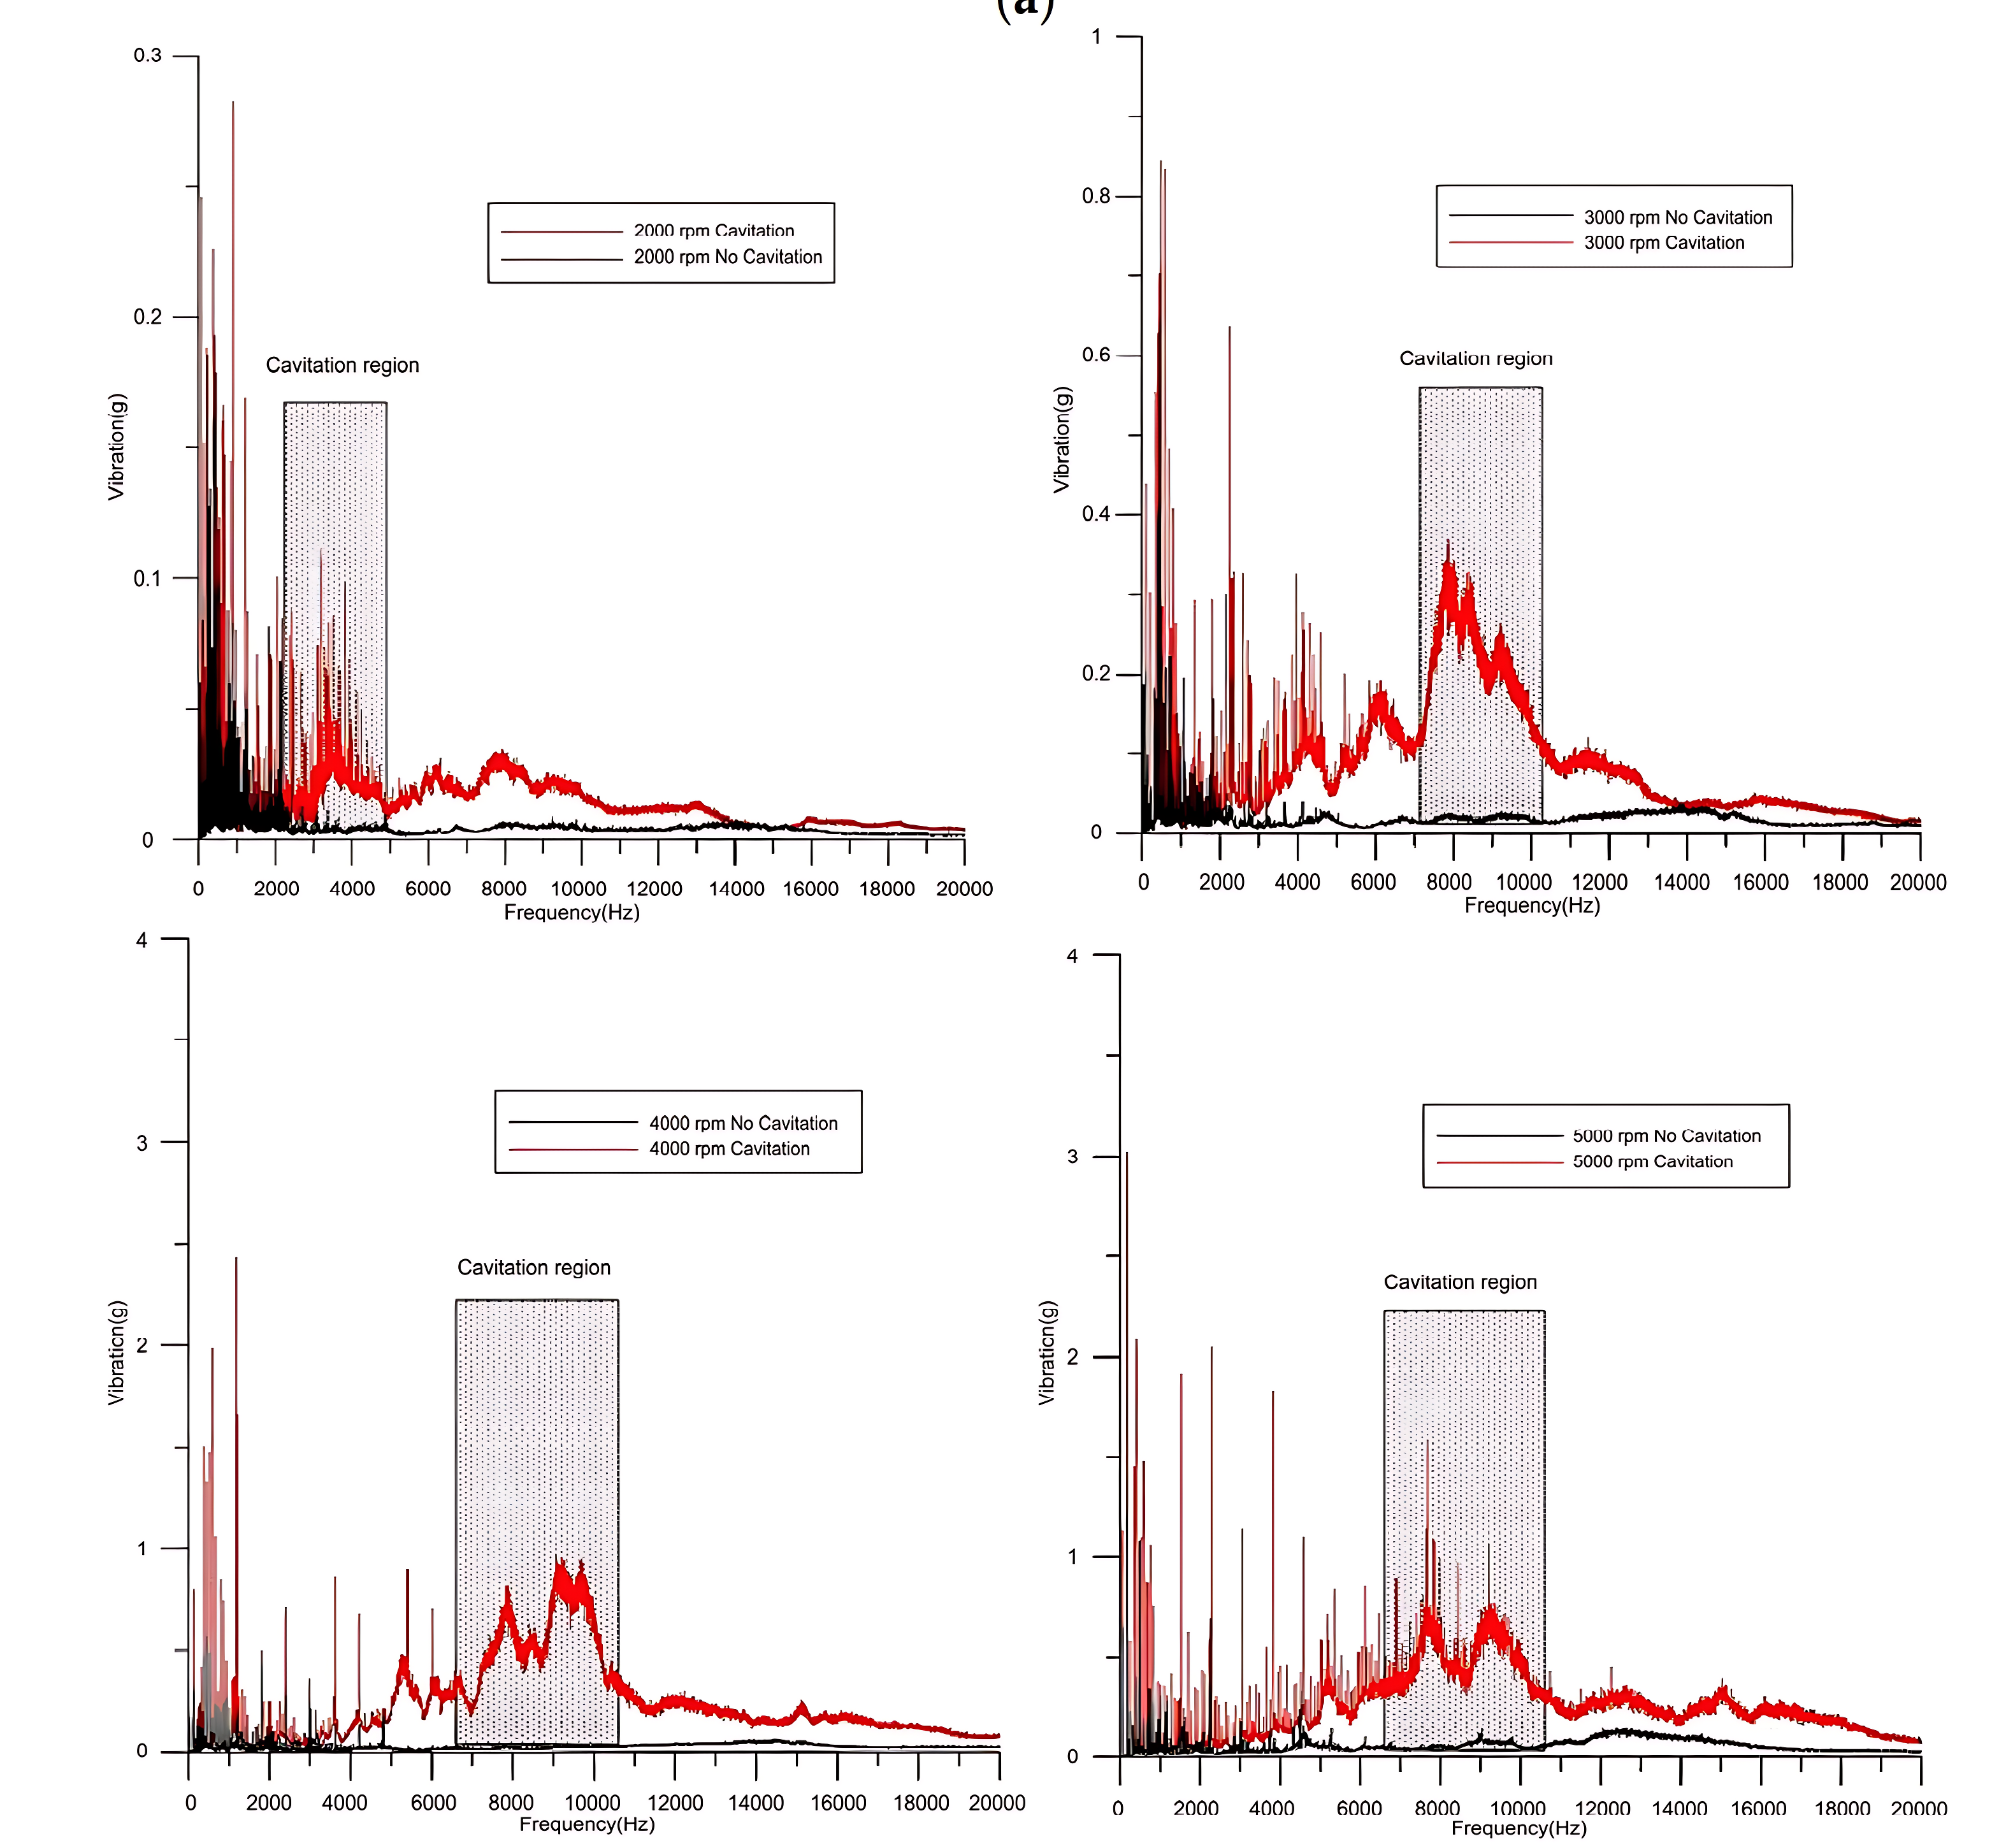
\includegraphics[width=0.95\linewidth]{figs//Artigos//Liu/Figura4B_Upscaler_4K.png}
    \caption{Espectro de sinal de vibração sob diferentes rpm. Fonte: \citeonline{liu2023review}}
    \label{fig:LiuFig4B}
\end{figure}

\linespread{1.27}\selectfont
Na Figura \ref{fig:LiuFig4B}, os sinais de vibração são analisados no domínio da frequência para diferentes velocidades de rotação (2000, 3000, 4000 e 5000 rpm). Os gráficos demonstram que, conforme a rotação aumenta, há um deslocamento e uma intensificação das componentes espectrais na faixa de 2 kHz a 8 kHz — região marcada como \textit{cavitation region}. Esses picos adicionais resultam da energia liberada pelos colapsos das bolhas de vapor, que introduzem novas componentes de alta frequência no espectro. A Figura \ref{fig:LiuFig4B} também mostra que a amplitude dessas componentes cresce com o aumento da rotação, evidenciando uma correlação direta entre a intensidade da cavitação e o conteúdo de alta frequência do sinal. Essa observação reforça a utilidade da análise espectral na \mbox{identificação e quantificação do fenômeno.}
\linespread{1.25}\selectfont

\begin{figure}[H]
    \centering
    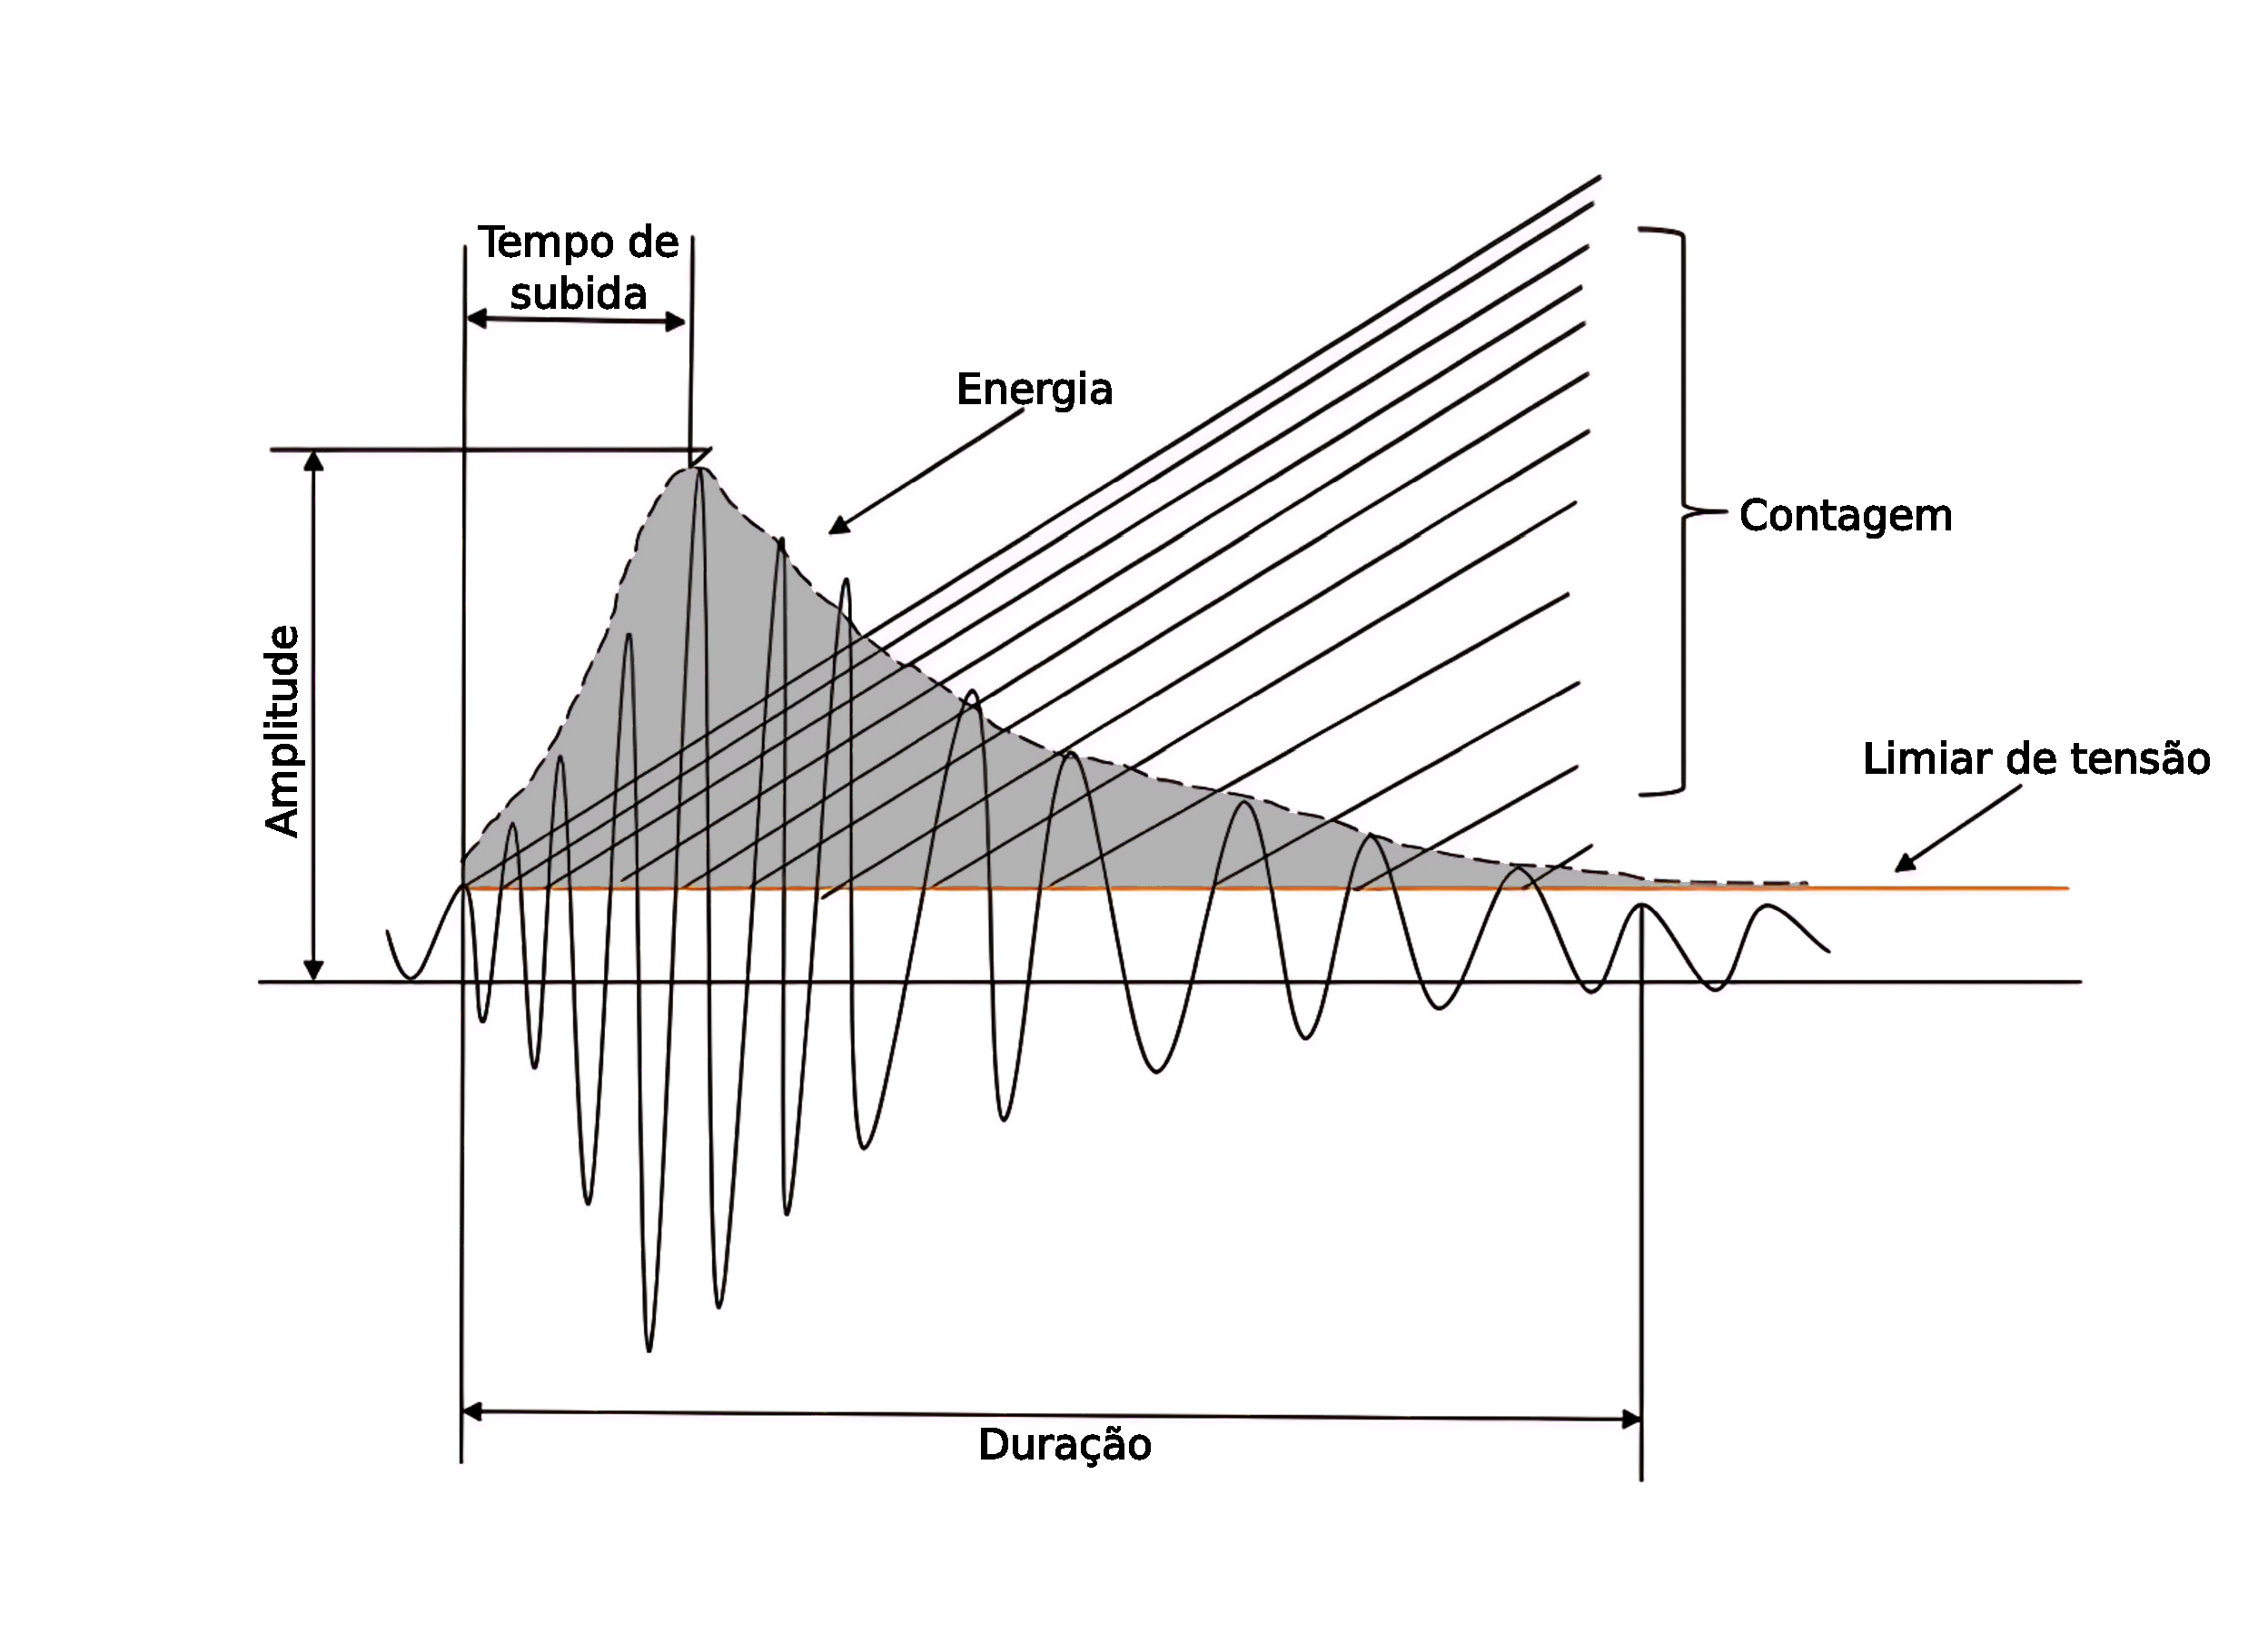
\includegraphics[width=0.9\linewidth]{figs//Artigos//Liu/Figura6.pdf}
    \caption{Parâmetros característicos do sinal de emissão acústica. Adaptado de  \citeonline{liu2023review}}
    \label{fig:LiuFig6}
\end{figure}

A Figura \ref{fig:LiuFig6} ilustra a decomposição de um evento típico de emissão acústica (“hit”) em seus principais parâmetros: amplitude, tempo de subida, \textit{rise time}, duração, energia e número de contagens acima do limiar, \textit{counts}. A amplitude representa o pico máximo do sinal, enquanto o tempo de subida corresponde ao intervalo entre o primeiro cruzamento do limiar e o pico máximo. A duração cobre o período total em que o sinal permanece acima do limiar, e a energia é obtida pela integral do sinal retificado. O número de contagens indica quantas vezes o sinal cruza o limiar estabelecido. Esses parâmetros são amplamente utilizados na caracterização de eventos de cavitação, pois refletem a intensidade e a frequência dos impactos associados ao colapso das bolhas, permitindo discriminar entre ruído e atividade cavitante real.

O ruído hidrodinâmico caracteriza-se por apresentar um espectro de banda larga e comportamento estocástico, resultante dos fenômenos de formação, crescimento e colapso de bolhas de vapor no interior do escoamento. Diferentemente do ruído mecânico, que tem natureza periódica e está associado a elementos estruturais da bomba (como mancais, rolamentos e pás do impulsor), o ruído hidrodinâmico reflete diretamente a instabilidade do fluido e as flutuações de pressão induzidas pela cavitação.

A Figura \ref{fig:LiuFig7}, adaptada de \citeonline{liu2023review}, apresenta a composição do ruído em bombas centrífugas, discriminando suas origens e mecanismos de formação. No topo, o ruído total da bomba, \textit{Pump noise} é dividido em dois grandes grupos: o ruído mecânico e o ruído hidrodinâmico. O primeiro engloba vibrações estruturais e ruídos discretos de frequência bem definida, como as frequências de passagem de pás e harmônicos, enquanto o segundo abrange componentes de ruído de cavitação, fluxo turbulento e separação de fluxo, de natureza predominantemente aleatória e de banda larga. Dentro do ruído de cavitação, por sua vez, distinguem-se componentes discretos e de banda larga, correspondentes a diferentes estágios e intensidades do fenômeno.

\begin{figure}[H]
\centering
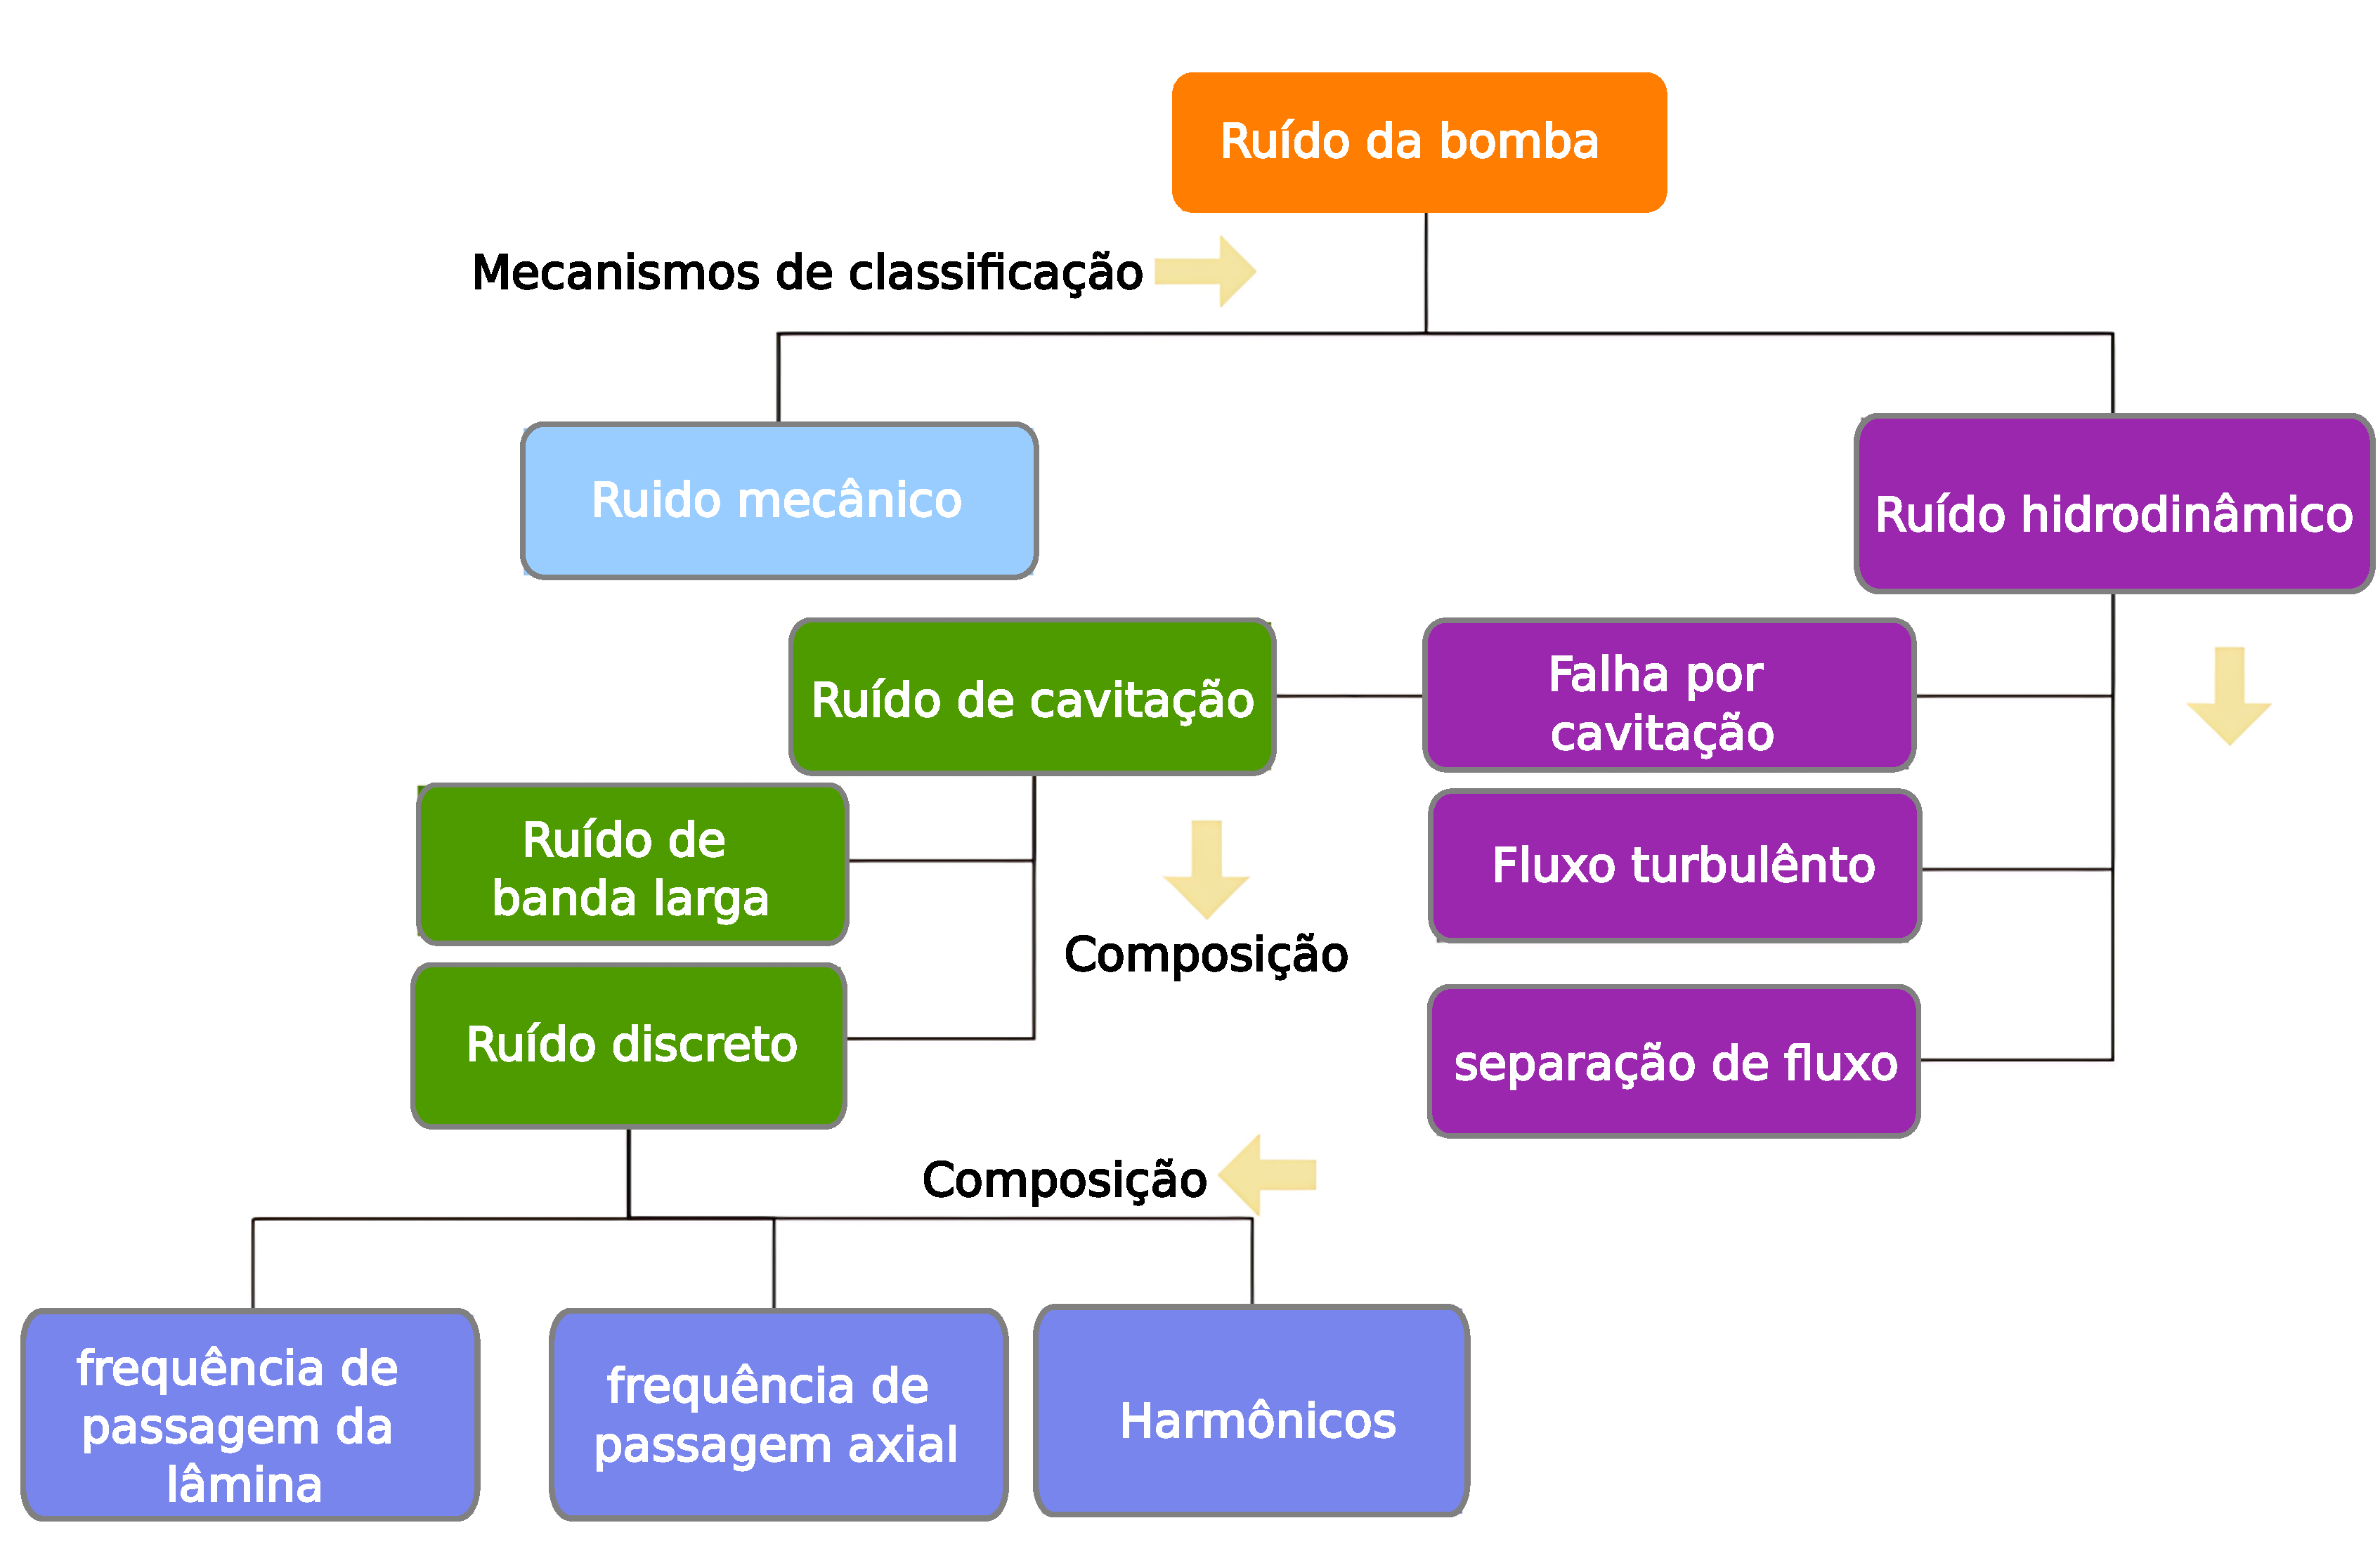
\includegraphics[width=0.75\linewidth]{figs//Artigos//Liu/Figura7.pdf}
\caption{Composição e mecanismos geradores do ruído em bombas centrífugas. Adaptado de \citeonline{liu2023review}.}
\label{fig:LiuFig7}
\end{figure}

Essa técnica de análise de ruído é particularmente útil em ensaios laboratoriais e ambientes controlados, nos quais as fontes de interferência externa podem ser minimizadas. Todavia, em aplicações industriais, sua eficácia tende a ser reduzida devido à forte influência de ruídos ambientais e à dificuldade de isolar as componentes específicas~associadas~à~cavitação.

Em contrapartida, o método baseado na pulsação de pressão apresenta maior robustez frente a interferências, uma vez que mede diretamente as variações de pressão no fluido, refletindo as flutuações hidráulicas e a eficiência volumétrica do sistema. Seu principal inconveniente, entretanto, é a natureza invasiva da instrumentação, que requer conexão física com o circuito hidráulico, além de uma baixa sensibilidade temporal para eventos de curta duração — o que limita sua capacidade de detectar a cavitação incipiente.

De modo comparativo, \citeonline{liu2023review} destacam que a emissão acústica e o ruído hidrodinâmico se sobressaem na detecção inicial da cavitação, enquanto a vibração é amplamente utilizada pela maturidade teórica e a pulsação de pressão pela robustez e simplicidade de implementação. As tendências futuras apontam para a convergência entre sensores de alta sensibilidade e métodos modernos de processamento de sinais não estacionários, aliada ao uso de inteligência artificial, em especial redes neurais convolucionais e aprendizado por reforço profundo, \mbox{para extração de padrões e detecção automatizada.}

Em síntese, a revisão conduzida por \citeonline{liu2023review} reforça que a emissão acústica permanece como uma das técnicas mais promissoras para a detecção precoce da cavitação, ainda que sua ampla adoção dependa de avanços em aspectos técnicos e econômicos, incluindo a redução de custos dos sensores piezoelétricos, a integração com hardware embarcado e o desenvolvimento de algoritmos otimizados para análise em tempo real.

\citeonline{poddar2021classification} apresentam um estudo voltado à detecção de falhas incipientes em mancais hidrodinâmicos, \textit{journal bearings}, investigando simultaneamente sinais EA e de vibração. Os autores ressaltam que fenômenos como cavitação, contaminação por partículas e falta de lubrificação são causas relevantes de degradação na performance de mancais, podendo levar à erosão, perda de eficiência e falhas prematuras. Neste contexto, métodos que permitam a identificação precoce dessas condições assumem papel crucial em estratégias de manutenção preditiva.

O experimento baseia-se em um arranjo monitorado, onde sensores de vibração e sensores de emissão acústica foram instalados em um mancal submetido a diferentes condições operacionais — incluindo variações no regime de carga, contaminação por partículas de diferentes tamanhos e situações de lubrificação insuficiente. O objetivo central consistiu em comparar a sensibilidade das duas técnicas, especialmente no que tange à detecção da cavitação incipiente. Os sinais coletados foram processados nos domínios do tempo e da frequência, a partir dos quais foram extraídos parâmetros como RMS, fator de crista, amplitude de pico, energia acumulada e número de contagens (no caso da EA). A análise foi estendida ao domínio tempo-frequência para capturar a \mbox{evolução espectral dos fenômenos de falha.}

Os resultados demonstram que os sinais de vibração apresentaram alterações significativas apenas em estágios mais avançados dos defeitos, quando ocorreram instabilidades acusadas no escoamento ou deterioração clara da película hidráulica. Em contraste, os sinais de emissão acústica revelaram-se muito mais sensíveis em estágios iniciais; observou-se, por exemplo, crescimento progressivo dos parâmetros energia acumulada e número de contagens com o agravamento da condição, o que evidencia uma correlação direta com os eventos de colapso de bolhas ou microcontatos. Os autores também apontam que amplitude e largura de banda dos sinais EA expandem-se de modo notável sob condições de falha — enquanto os índices de vibração \mbox{mantêm-se relativamente estáveis.}

A discussão conclui que a técnica de emissão acústica apresenta desempenho claramente superior na detecção precoce da cavitação e de deteriorações relacionadas, pois consegue identificar alterações no regime de escoamento antes mesmo que se verifique qualquer impacto mensurável no desempenho hidrodinâmico global do equipamento. A análise vibracional, embora útil, tende a ser mais responsiva em estágios posteriores da falha, quando modificações estruturais ou oscilações adicionais já se refletem na resposta dinâmica do conjunto. Do ponto de vista metodológico, o estudo indica que a integração entre ambas as abordagens pode enriquecer o diagnóstico, ampliando a compreensão do processo de degradação. Contudo, mesmo sem recorrer a medições complementares, a EA já se mostra como a alternativa mais sensível e promissora para a identificação incipiente de cavitação, conforme evidenciado em \citeonline{poddar2021classification}.

\citeonline{amini2022development} apresentam o desenvolvimento de um sistema inovador para o monitoramento da cavitação em turbinas hidráulicas, fundamentado na análise de sinais acústicos aliada a algoritmos de aprendizado de máquina. Os autores apontam que a operação de turbinas em condições fora do ponto ótimo de eficiência aumenta a probabilidade de ocorrência de cavitação, o que por sua vez acarreta degradação de desempenho, vibrações estruturais e, principalmente, danos mecânicos por erosão. Nesse sentido, a proposta busca oferecer uma ferramenta não intrusiva, capaz de detectar tanto a ocorrência quanto a severidade do fenômeno em tempo real, contribuindo para a manutenção preditiva em centrais hidrelétricas.

A metodologia foi organizada em duas fases distintas. Na primeira, foram realizados experimentos controlados no túnel de cavitação da HES-SO Valais/Wallis, em que se utilizou um hidrofólio de aço inoxidável do tipo NACA 0015 para induzir a cavitação em condições estáticas e dinâmicas, conforme ilustrado na Figura \ref{fig:amini2022developmentFig1}. Nessa etapa, o ruído no aerofólio foi registrado por meio de um microfone GRAS 46 AE com frequência de amostragem de 40 kHz, e os sinais foram analisados nos domínios temporal e espectral. Em uma segunda fase, a técnica foi validada em escala real na usina hidrelétrica de Ernen, no cantão de Valais (Suíça), equipada com turbinas Francis de 16 MW cada, como mostra a Figura \ref{fig:amini2022developmentFig2}. Durante essa campanha experimental, foram simuladas diferentes condições operacionais, abrangendo variações de carga, níveis de jusante e introdução de ruídos artificiais, com o intuito de avaliar a robustez do sistema.

\begin{figure}[H]
    \centering
    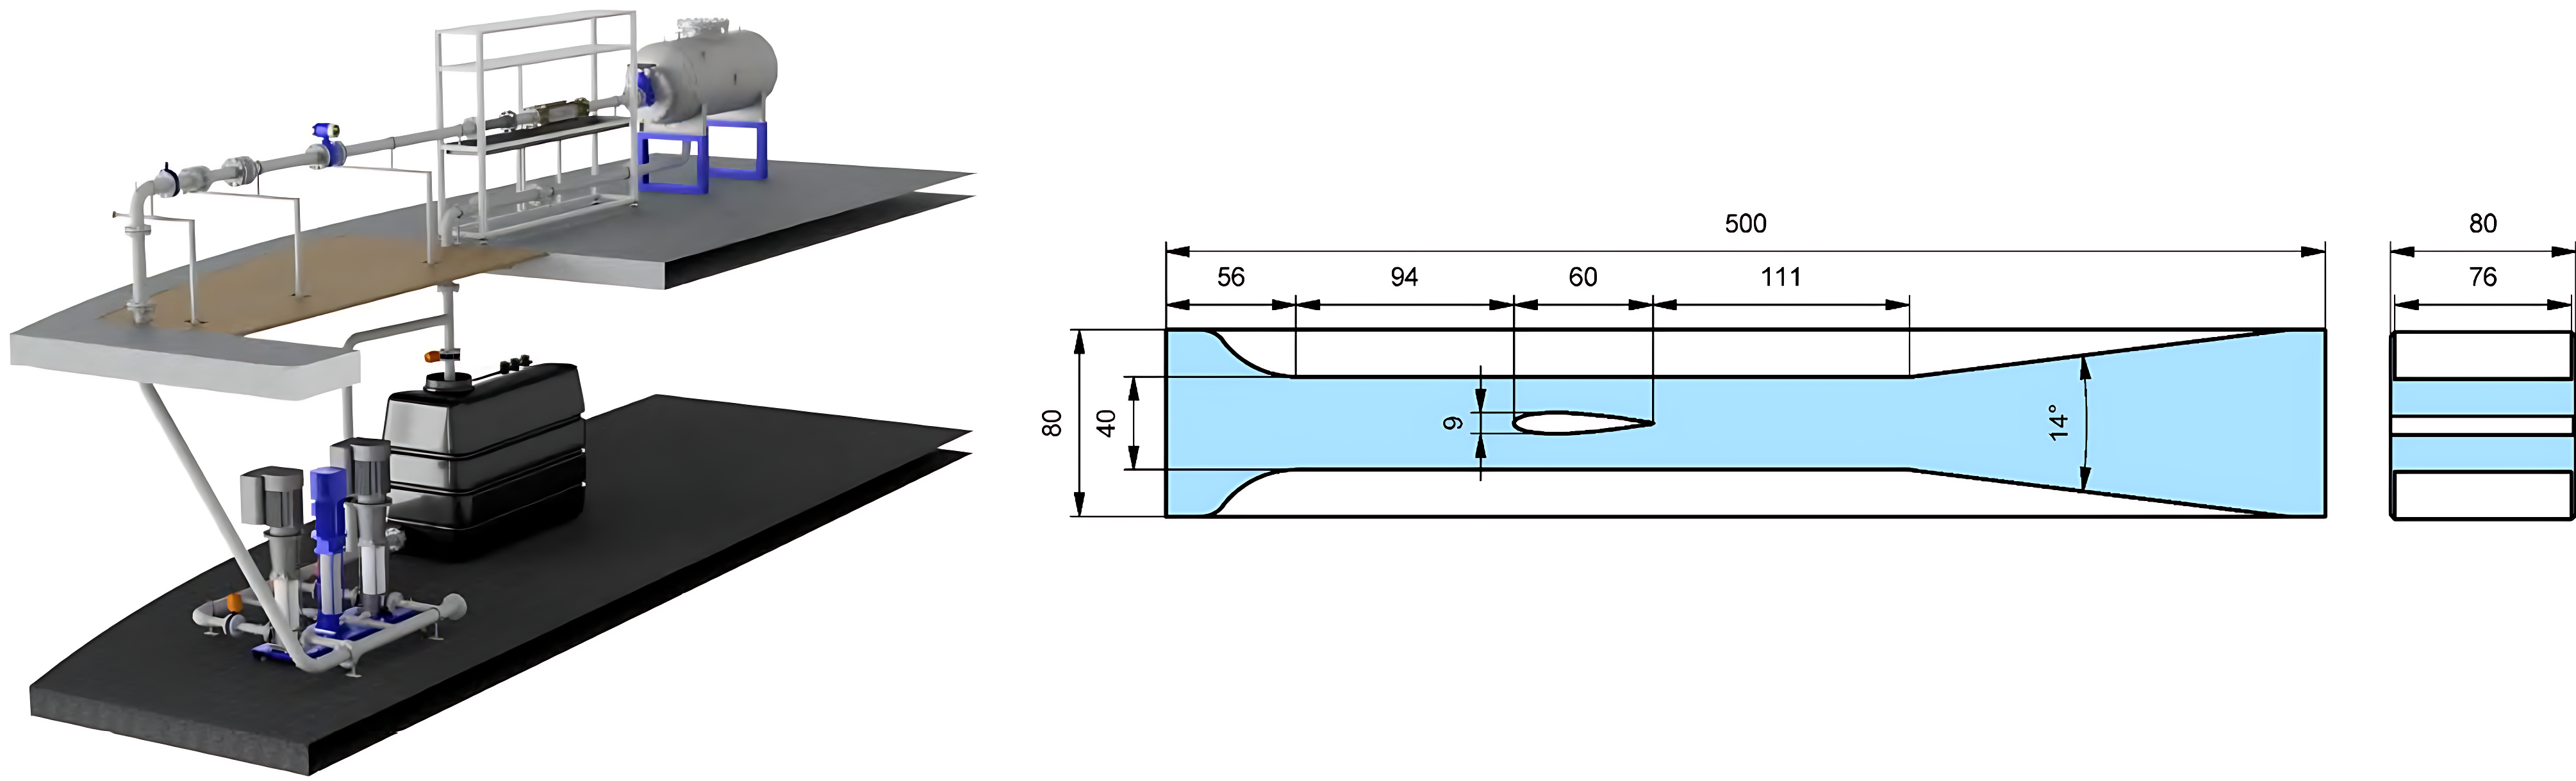
\includegraphics[width=1.0\linewidth]{figs/Artigos/amini2022development/Figura1_Upscaler_2K.png}
    \caption{(À esquerda) esquema do túnel de cavitação da HES-SO Valais/Wallis; (À direita) seção transversal do hidrofólio de aço inoxidável NACA 0015 testado. Fonte: \citeonline{amini2022development}}
    \label{fig:amini2022developmentFig1}
\end{figure}

\begin{figure}[H]
    \centering
    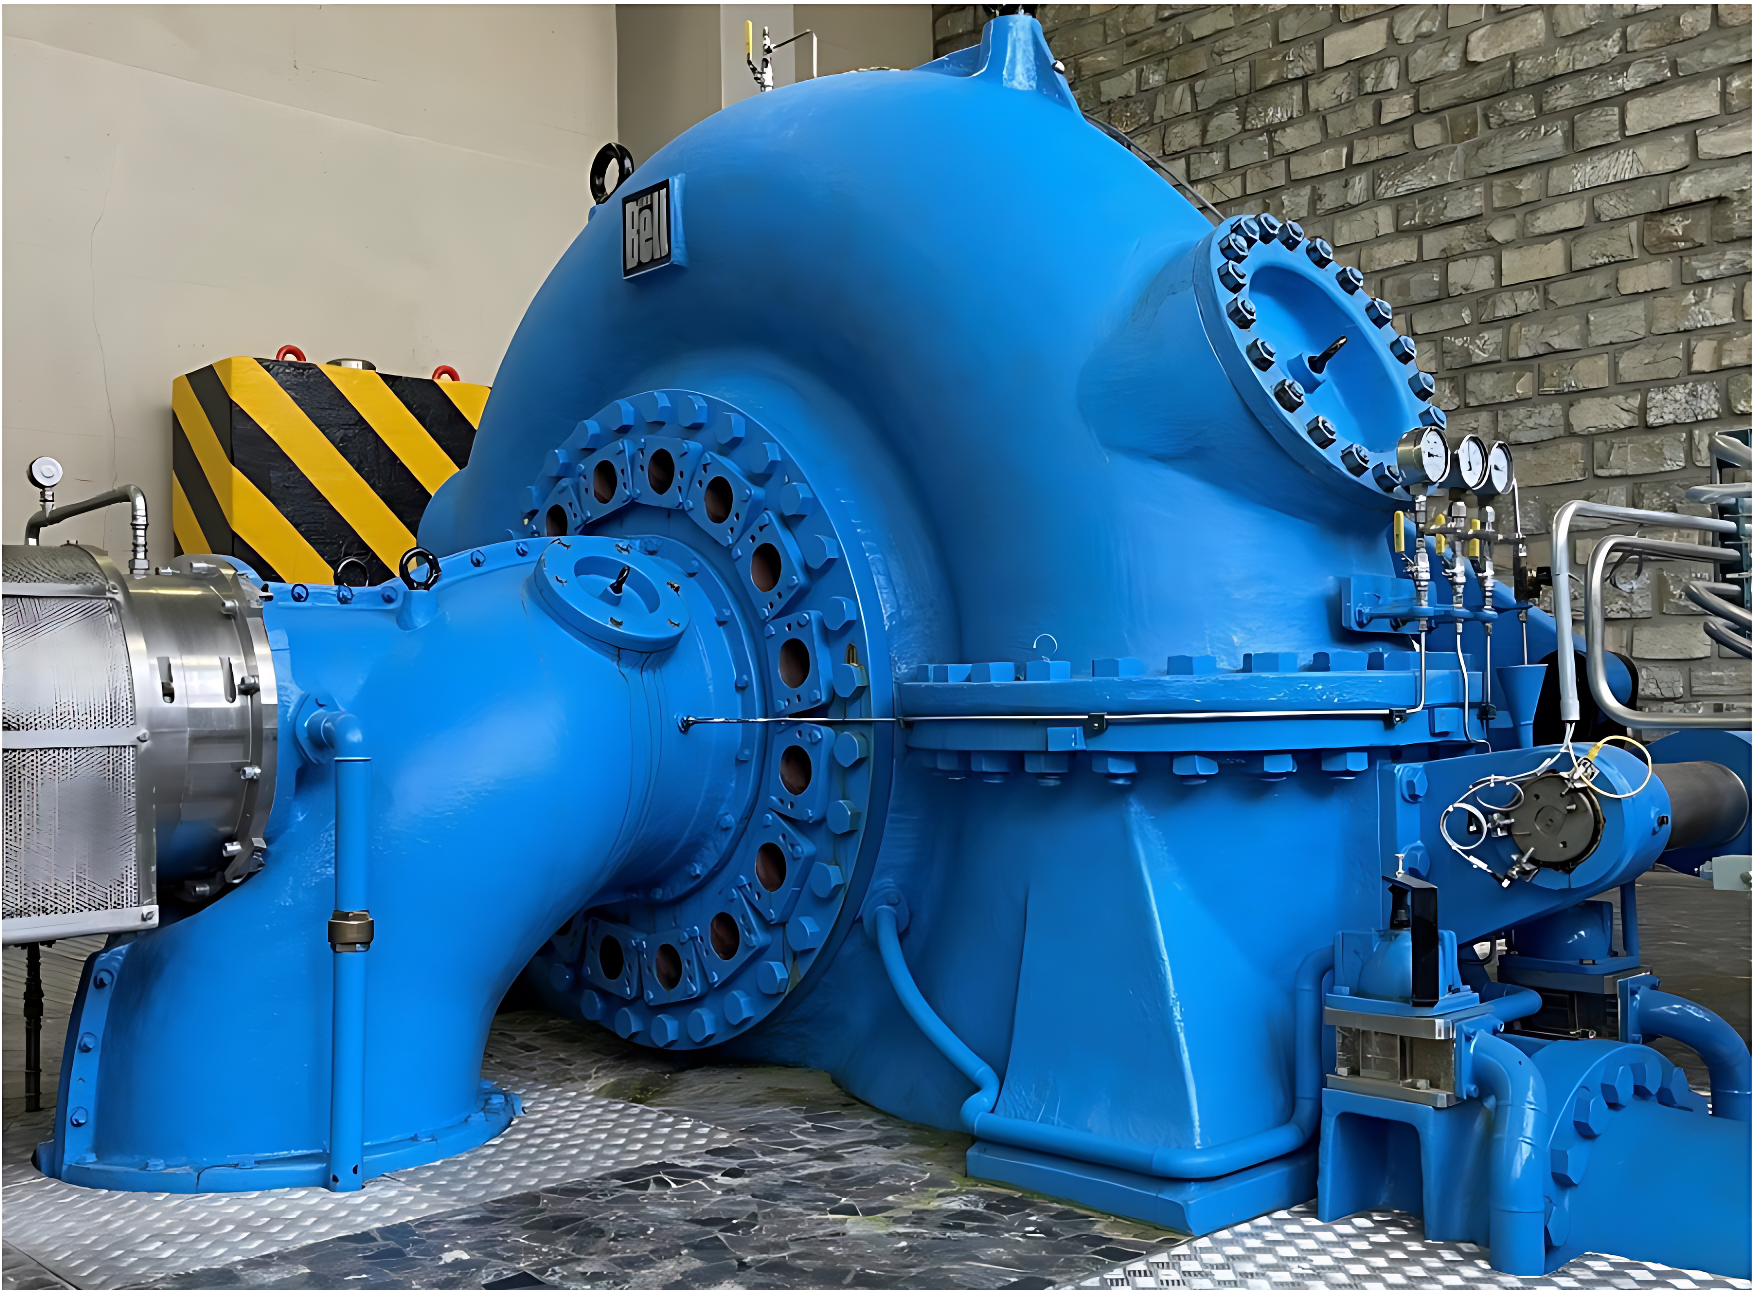
\includegraphics[width=.85\linewidth]{figs/Artigos/amini2022development/Figura2_Upscaler_2K.png}
    \caption{Turbina Francis de dois rotores na usina hidrelétrica de Ernen (Wallis, Suíça). Fonte: \citeonline{amini2022development}}
    \label{fig:amini2022developmentFig2}
\end{figure}

\linespread{1.27}\selectfont
As figuras explicam por si o salto metodológico:  
Figura \ref{fig:amini2022developmentFig1}: ilustra a instalação experimental de bancada no túnel de cavitação, onde o hidrofólio NACA 0015 foi submetido a perfis de escoamento com pressão de sucção reduzida para induzir cavitação. O desenho da seção transversal do hidrofólio permite visualizar as dimensões e geometria usadas nos testes. Essa figura demonstra claramente a etapa de laboratório, onde as condições são controladas, permitindo análise precisa dos sinais acústicos captados.

Figura \ref{fig:amini2022developmentFig2}: apresenta a aplicação em campo real, com uma turbina Francis de dois rotores na usina de Ernen. Essa imagem reforça a transição da metodologia do laboratório para o ambiente operacional industrial, destacando a compatibilidade da solução desenvolvida com sistemas de grande escala. A capacidade de validação em usina real confere maior credibilidade à técnica proposta.  

Em resumo, o estudo reforça a viabilidade do uso de sinais acústicos não invasivos em combinação com algoritmos de aprendizado para o monitoramento da cavitação em turbinas hidráulicas. A abordagem — centrada em microfones, processamento de sinais e classificação supervisionada — fornece uma estrutura promissora para aplicações industriais, o que dialoga diretamente com o foco desta dissertação: a implementação simulada de uma rede neural de convolução (CNN-1D) em hardware reconfigurável (FPGA) para detecção de falhas em sistemas hidráulicos.

\linespread{1.27}\selectfont
O processamento dos sinais foi realizado por meio da transformada rápida de Fourier (FFT) e da extração de características no domínio da frequência, com o objetivo de identificar padrões representativos da cavitação. Para a etapa de classificação supervisionada, foram testados dois algoritmos de aprendizado de máquina: o \textit{k-Nearest Neighbors} (k-NN), aplicado aos ensaios laboratoriais, e o \textit{Gaussian Mixture Model} (GMM), utilizado para os dados coletados na usina. 

Os resultados mostraram que, em condições estáticas de laboratório, a distinção entre regimes cavitantes e não cavitantes foi clara, atingindo 100\% de acurácia. Já nos ensaios dinâmicos, a precisão manteve-se elevada, superior a 95\%, mesmo diante da maior complexidade imposta pela rotulagem de dados e pela ausência de critérios visuais diretos para validação, como ilustram as Figuras~\ref{fig:amini2022developmentFig3} e~\ref{fig:amini2022developmentFig4}. Na aplicação em escala real, apesar da presença de ruído de fundo significativo, o algoritmo manteve desempenho consistente, separando com clareza as diferentes classes de operação e identificando distintos níveis de severidade da cavitação, conforme apresentado na Figura~\ref{fig:amini2022developmentFig6}.

\begin{figure}[H]
    \centering
    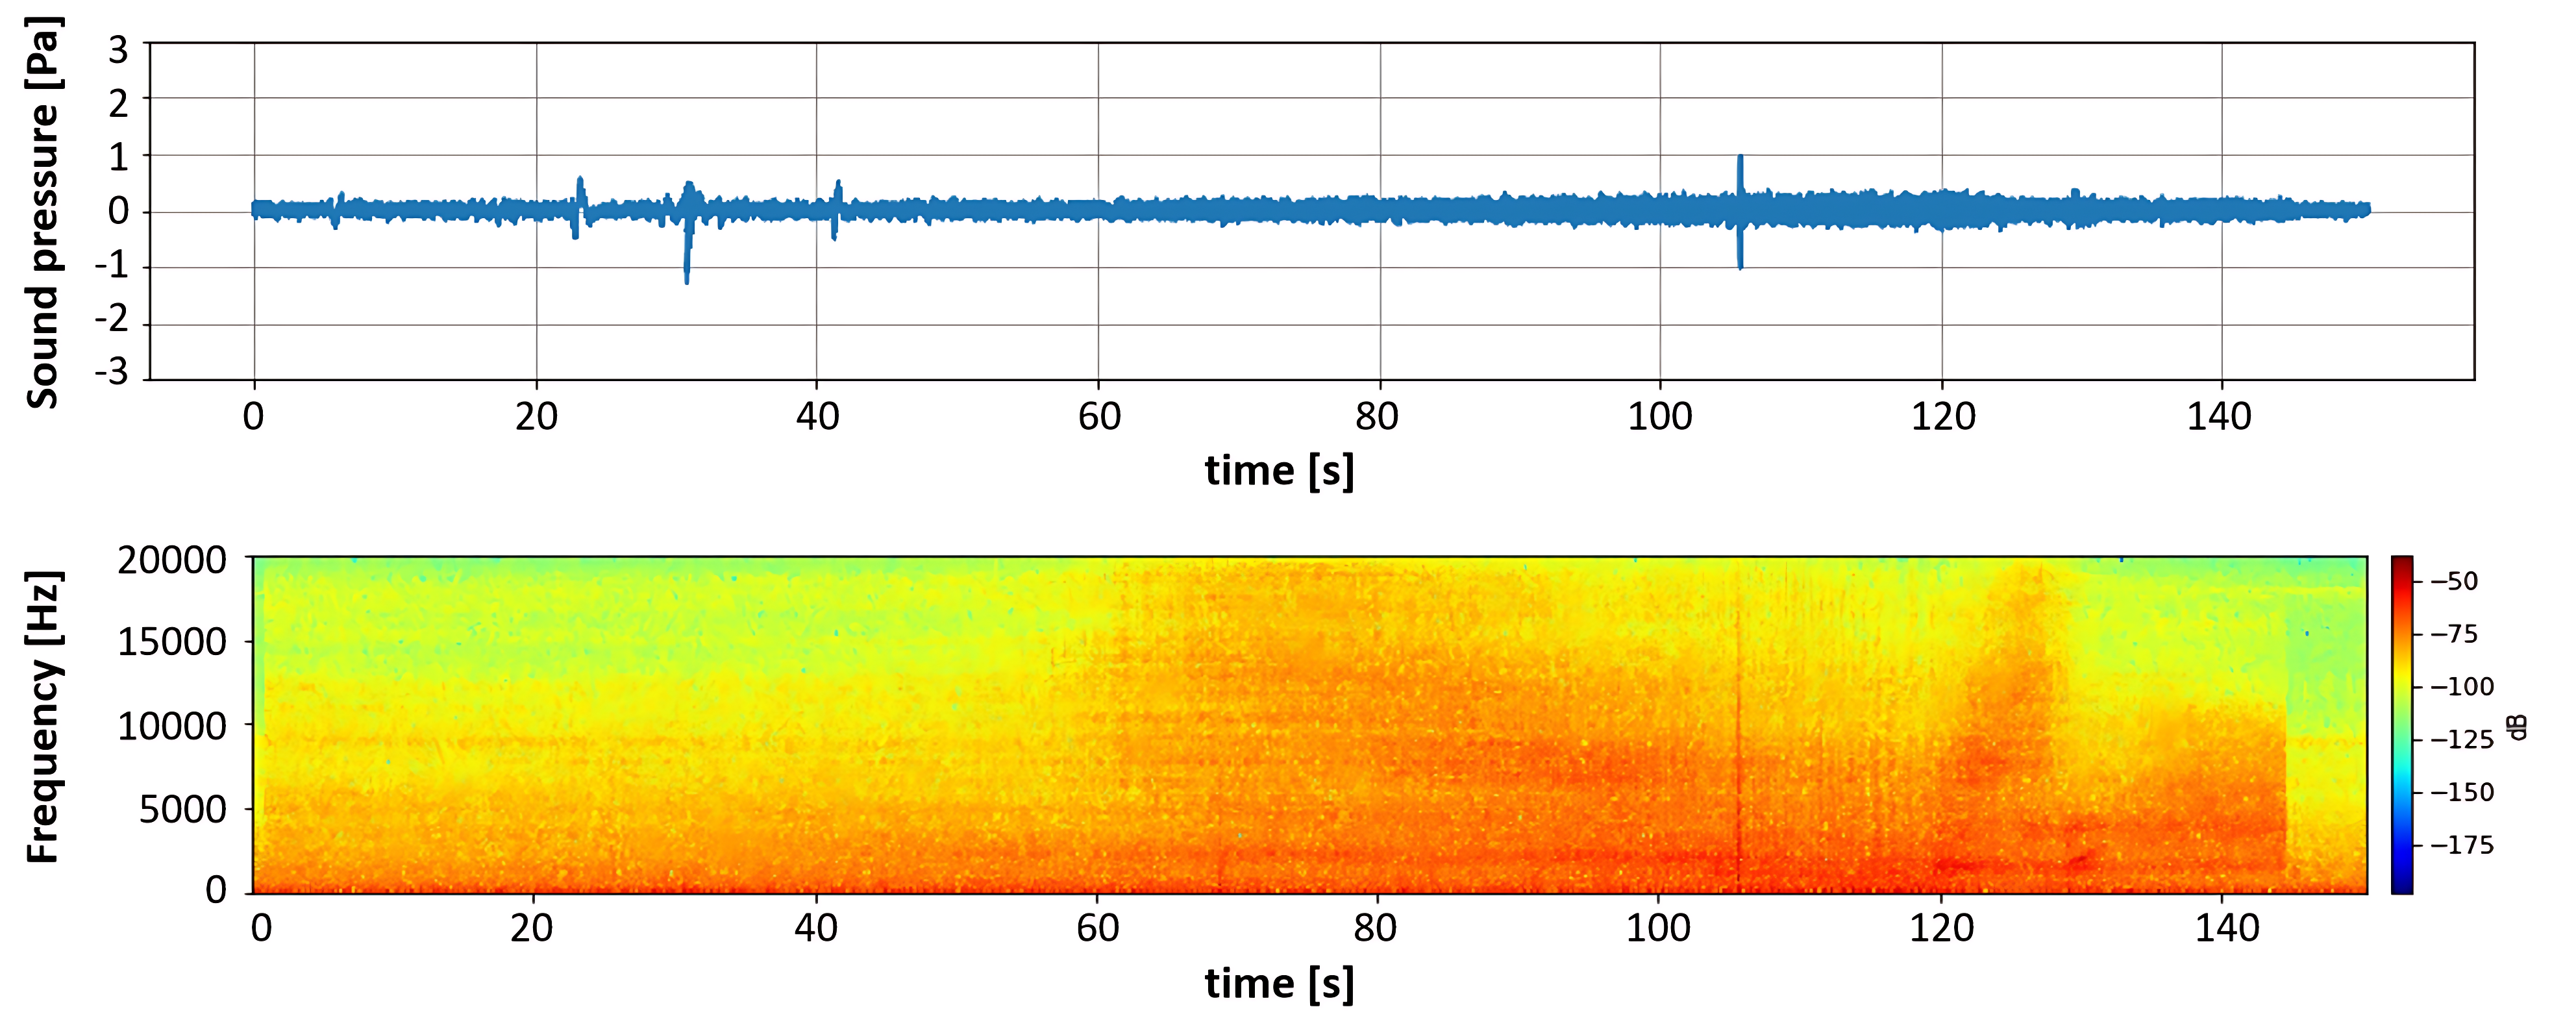
\includegraphics[width=1.0\linewidth]{figs/Artigos/amini2022development/Figura3_Upscaler_2K.png}
    \caption{Sinal acústico de um teste dinâmico ilustrado nos domínios de tempo (acima) e de frequência (abaixo). Fonte: \citeonline{amini2022development}}
    \label{fig:amini2022developmentFig3}
\end{figure}

\linespread{1.27}\selectfont
A Figura~\ref{fig:amini2022developmentFig3} apresenta o sinal acústico registrado durante um teste dinâmico. A parte superior mostra a variação da pressão sonora no tempo, enquanto o espectrograma inferior exibe a distribuição de energia no domínio da frequência. É possível observar o aumento de componentes de alta frequência à medida que a cavitação se intensifica, evidenciando a sensibilidade do método acústico.
\linespread{1.25}\selectfont

\begin{figure}[H]
    \centering
    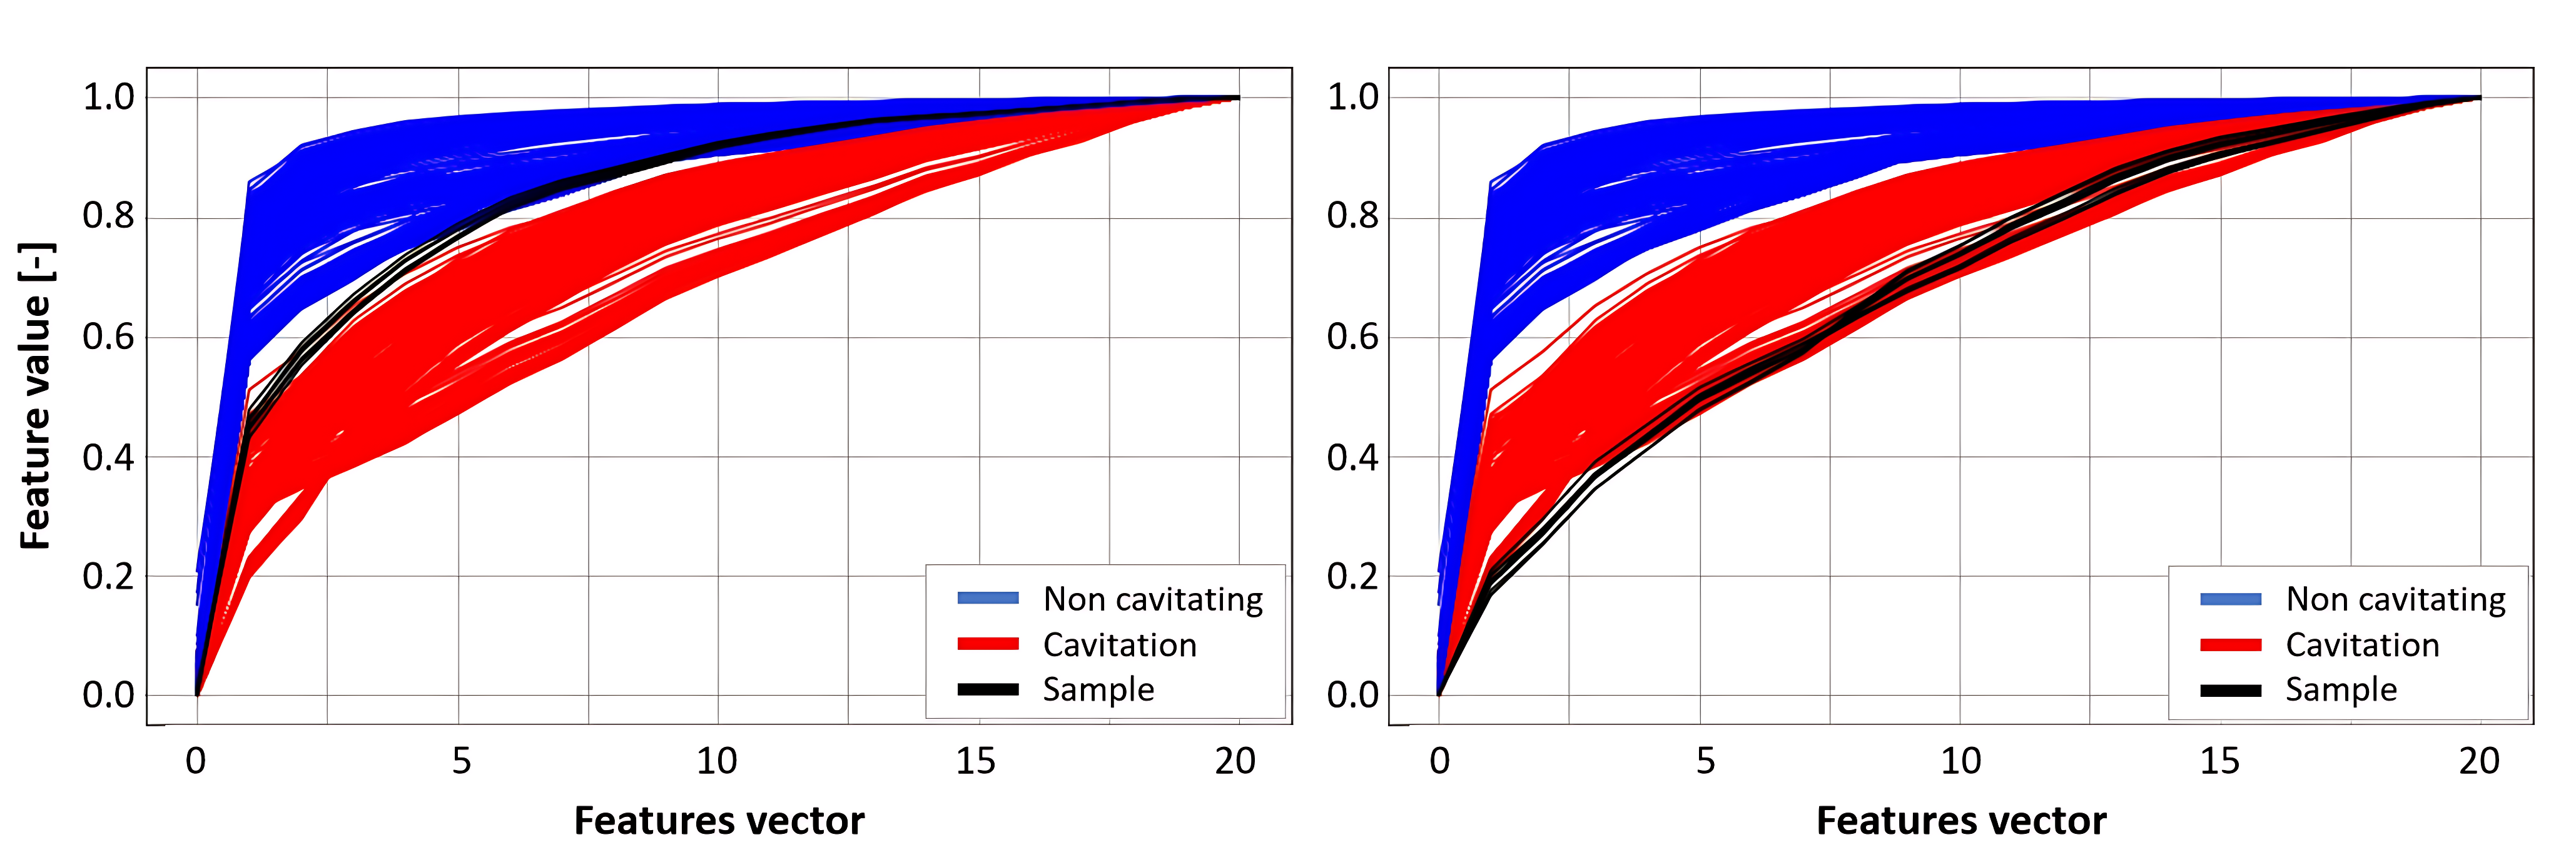
\includegraphics[width=1.0\linewidth]{figs/Artigos/amini2022development/Figura4_Upscaler_2K.png}
    \caption{Distribuição dos valores característicos extraídos dos sinais de ML para fluxos cavitantes (vermelho) e não cavitantes (azul), obtidos em testes estáticos com $\alpha = 8^\circ$. A curva preta à esquerda corresponde ao estado não cavitante em um teste dinâmico no mesmo ângulo, enquanto a curva à direita representa a condição cavitante sob o mesmo regime. Fonte: \citeonline{amini2022development}}
    \label{fig:amini2022developmentFig4}
\end{figure}

A Figura~\ref{fig:amini2022developmentFig4} mostra a distribuição das características extraídas dos sinais para diferentes condições de escoamento. Os fluxos cavitantes apresentam valores de atributos significativamente distintos dos não cavitantes, permitindo uma separação clara entre as classes. As curvas pretas destacam um teste dinâmico intermediário, demonstrando coerência entre as transições de regime.

\begin{figure}[H]
    \centering
    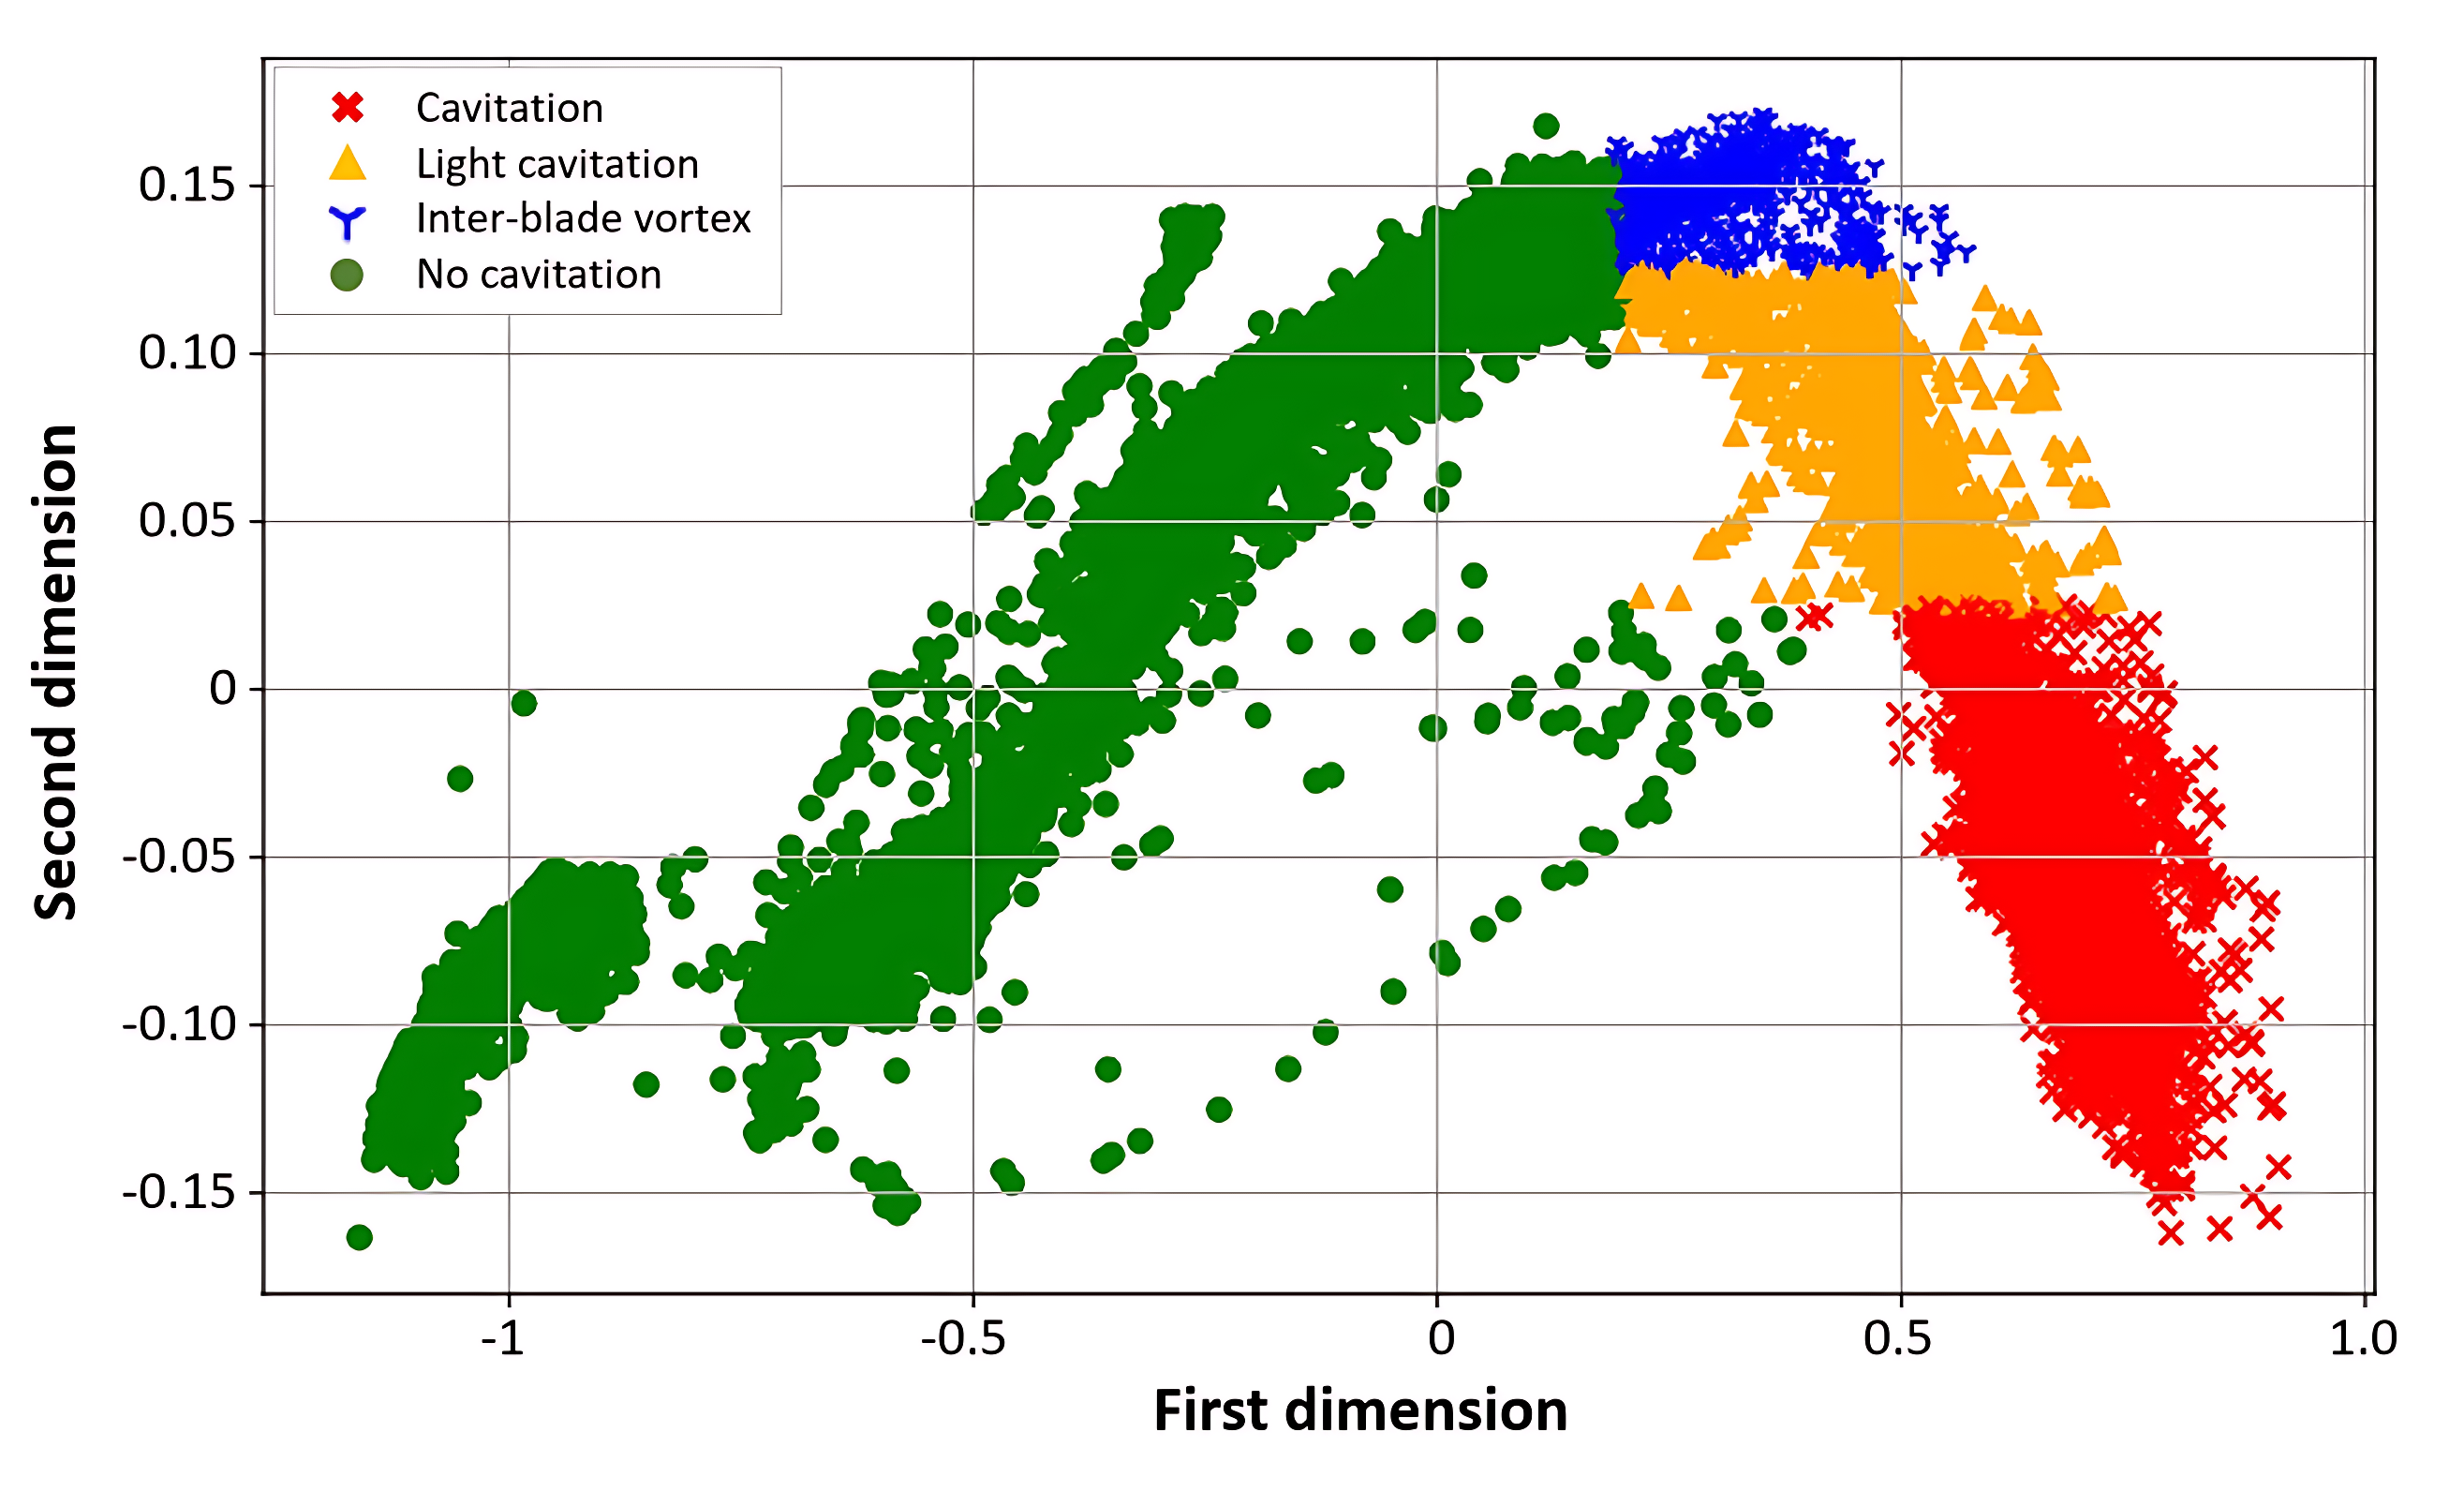
\includegraphics[width=.8\linewidth]{figs/Artigos/amini2022development/Figura6_Upscaler_2K.png}
    \caption{Projeção bidimensional dos dados de operação da turbina obtidos na usina de Ernen, classificando diferentes estados de escoamento: sem cavitação (verde), cavitação leve (amarelo), cavitação plena (vermelho) e vórtices interpalhetas (azul). Fonte: \citeonline{amini2022development}}
    \label{fig:amini2022developmentFig6}
\end{figure}
    
A Figura~\ref{fig:amini2022developmentFig6} exibe o resultado da classificação obtida no ambiente real da usina hidrelétrica. Cada ponto representa um vetor de características projetado em duas dimensões (via redução de dimensionalidade). Observa-se uma separação bem definida entre quatro condições: operação normal, cavitação leve, cavitação severa e presença de vórtices entre pás. Essa distinção confirma a robustez do modelo GMM, mesmo sob ruído operacional e variação de carga.

Em síntese, o estudo demonstra que a combinação entre processamento acústico e aprendizado de máquina é capaz de discriminar, com alta confiabilidade, diferentes estágios de cavitação tanto em condições laboratoriais quanto em ambiente industrial. Os resultados reforçam o potencial dessa abordagem para o monitoramento não intrusivo e o diagnóstico preditivo de turbinas hidráulicas.

Uma análise estatística complementar, realizada a partir do histórico operacional de sete anos da usina, revelou que as turbinas frequentemente operaram em faixas de carga parcial propensas à cavitação. Essa constatação sugere que o fenômeno pode ter contribuído para o desgaste prematuro de componentes e para a redução da eficiência global das máquinas, conforme apresentado na Figura~\ref{fig:amini2022developmentFig7}. Dessa forma, o sistema proposto pelos autores não apenas permite a detecção em tempo real, mas também possibilita o diagnóstico retrospectivo do número de horas em regime cavitante, ampliando seu potencial como ferramenta de manutenção preditiva.

\begin{figure}[H]
    \centering
    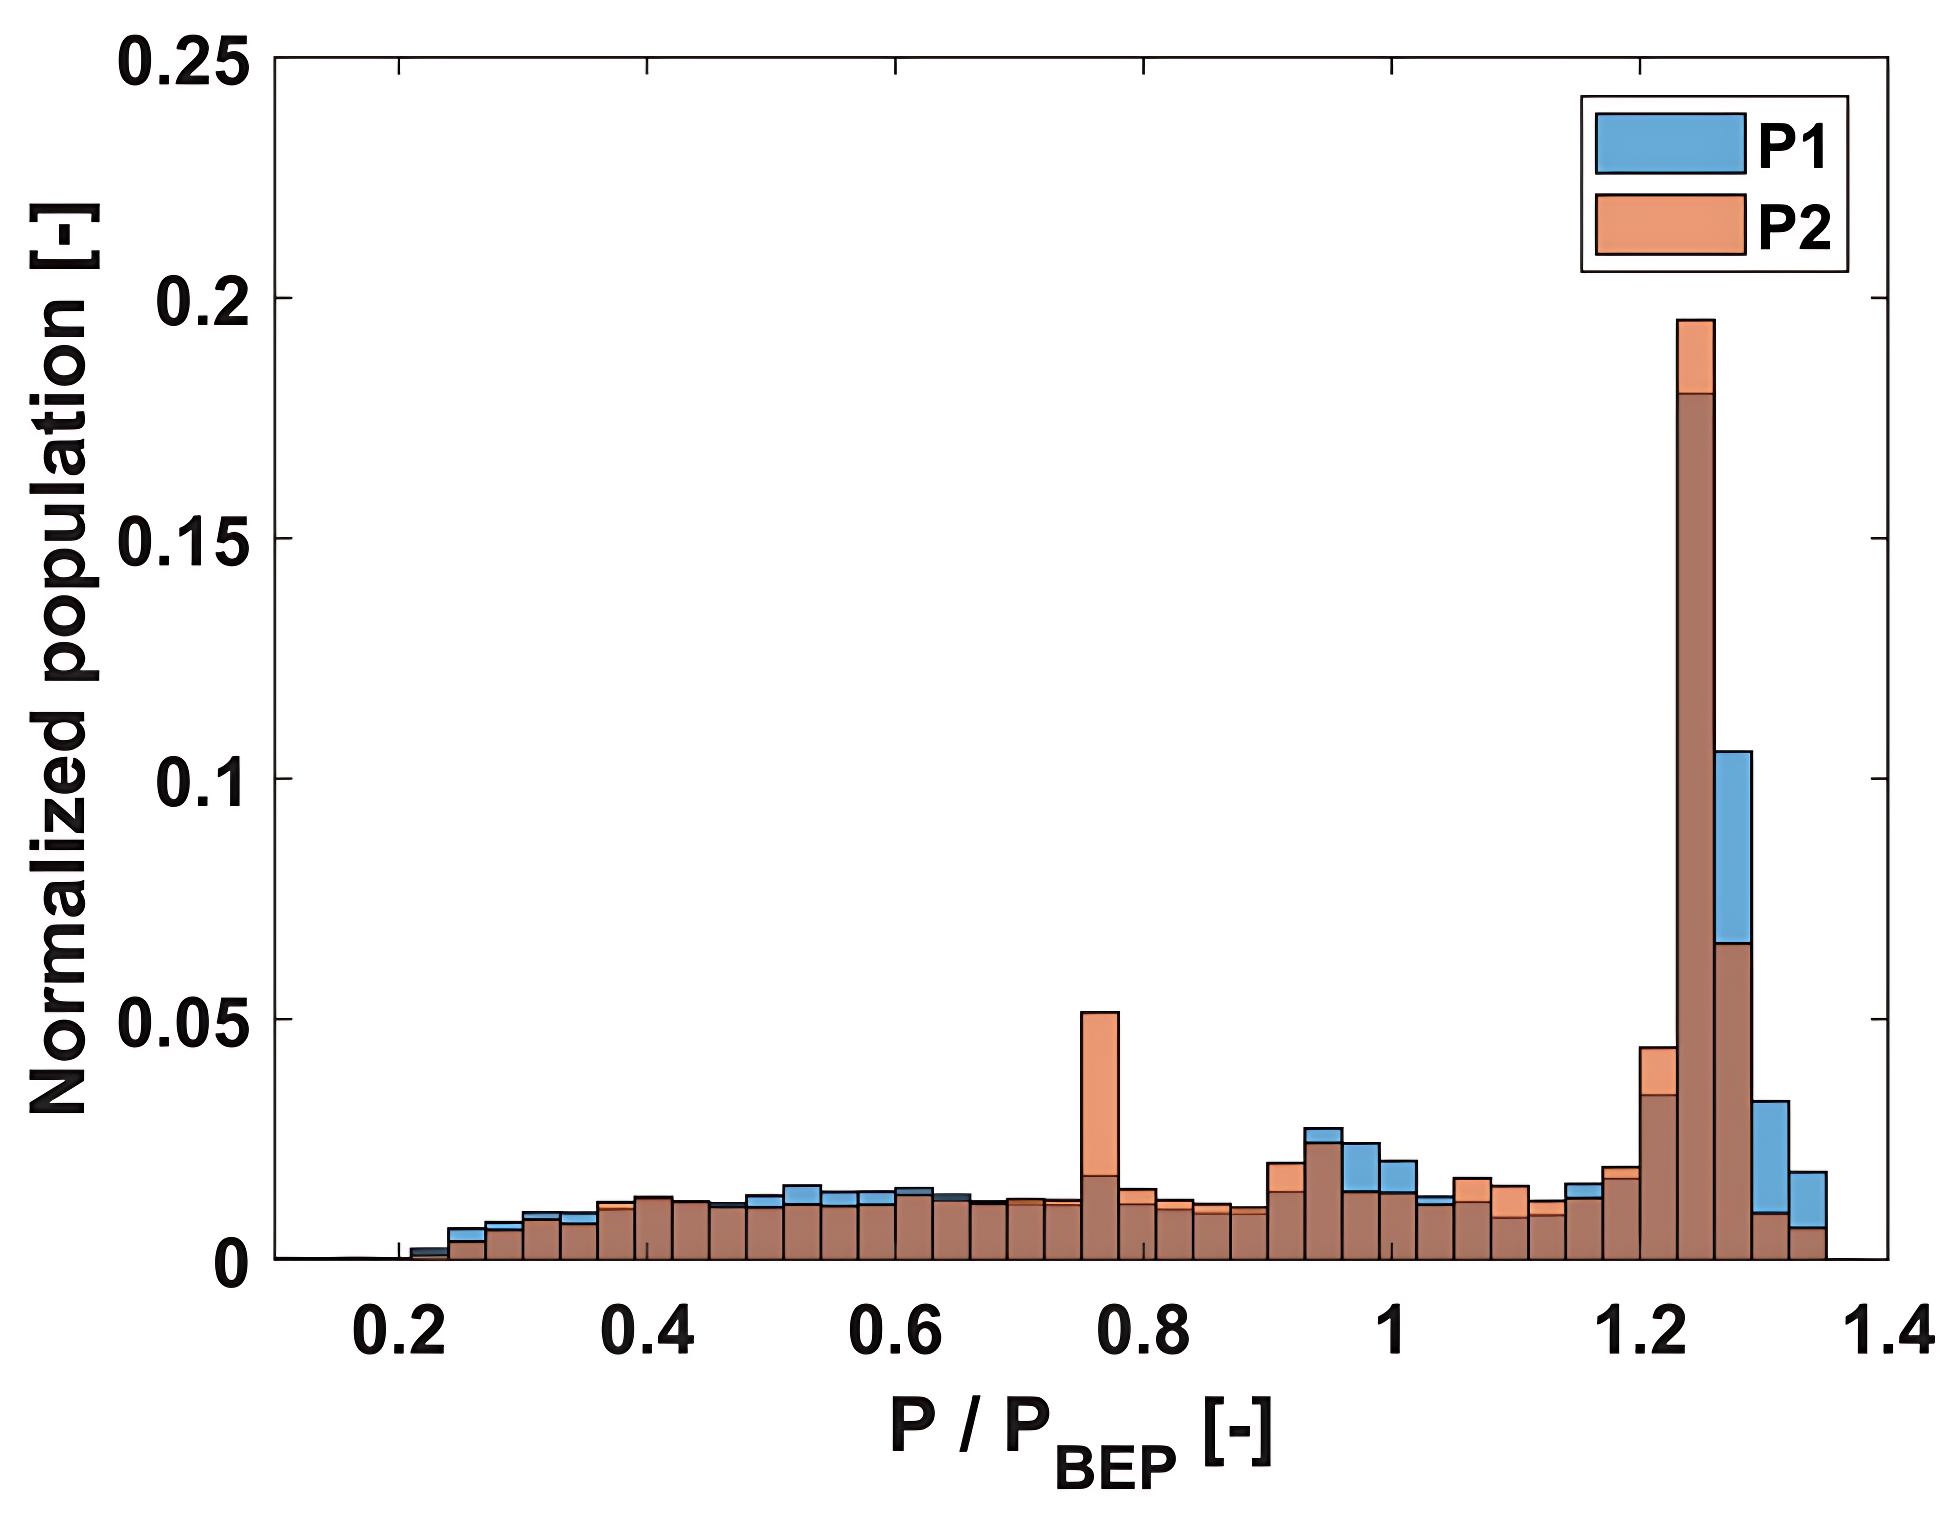
\includegraphics[width=.55\linewidth]{figs/Artigos/amini2022development/Figura7_Upscaler_2K.png}
    \caption{Distribuição normalizada da taxa de potência das duas turbinas idênticas (P1 e P2) da usina hidrelétrica de Ernen ao longo de um período de sete anos. Fonte: \citeonline{amini2022development}}
    \label{fig:amini2022developmentFig7}
\end{figure}

\linespread{1.28}\selectfont
A Figura~\ref{fig:amini2022developmentFig7} evidencia a frequência relativa de operação das duas turbinas, expressa em função da potência normalizada $P / P_{BEP}$, sendo $P_{BEP}$ a potência correspondente ao ponto de melhor eficiência \textit{Best Efficiency Point}. Observa-se que ambas as unidades operaram de forma recorrente acima de $1{,}2\,P_{BEP}$, faixa associada a maior risco de cavitação. Essa distribuição reforça a importância de sistemas de monitoramento contínuo, visto que períodos prolongados nesse regime podem causar erosão nas pás, vibrações excessivas e perdas de desempenho hidráulico. Além disso, a análise mostra a utilidade do sistema proposto não apenas para o acompanhamento em tempo real, mas também como ferramenta de avaliação histórica das condições operacionais e identificação de padrões de desgaste.

\linespread{1.28}\selectfont
Em conclusão, \citeonline{amini2022development} demonstram a viabilidade de um método não intrusivo para detecção de cavitação em turbinas hidráulicas, baseado em sinais acústicos e aprendizado de máquina. O sistema foi validado tanto em condições laboratoriais quanto em escala industrial, apresentando alta precisão na identificação de diferentes regimes de escoamento. Os autores ainda destacam o potencial de aprimoramento futuro por meio da incorporação de algoritmos mais avançados, capazes de distinguir entre diferentes tipos de cavitação e estimar índices de severidade. Tais avanços poderiam ser generalizados para outras configurações de turbinas mediante o uso de técnicas de aprendizado por transferência, ampliando o escopo de aplicação em sistemas hidrelétricos.

\linespread{1.28}\selectfont
A seguir, apresenta-se uma comparação sistemática dos principais tipos de sensores empregados na detecção de cavitação em bombas centrífugas, destacando suas faixas de frequência típicas, vantagens, limitações e aplicações mais adequadas. A Tabela \ref{tab:sensores_cavitacao} sintetiza essas características e proporciona ao leitor uma visão panorâmica dos trade-offs entre custo, sensibilidade e operacionalidade de cada sensor. Com isso, pretende-se facilitar a escolha adequada do sistema de medição conforme o estágio de cavitação, a criticidade do equipamento e o contexto de monitoramento industrial.

\begin{table}[H]
\footnotesize
\centering
\caption{Comparação entre diferentes tipos de sensores utilizados na detecção de cavitação em bombas centrífugas. Adaptado de \citeonline{liu2023review}.}
\label{tab:sensores_cavitacao}
\renewcommand{\arraystretch}{1.3}
\resizebox{\textwidth}{!}{%
\begin{tabular}{p{3.0cm} p{2.4cm} p{4.2cm} p{4.2cm} p{3.2cm}}
\hline
\textbf{Tipo de Sensor} & \textbf{Faixa típica de frequência} & \textbf{Vantagens principais} & \textbf{Limitações} & \textbf{Aplicações mais adequadas} \\ \hline

\textbf{Acelerômetro} &
1Hz – 20kHz &
Baixo custo, ampla disponibilidade e fácil instalação; fornece informações estruturais globais e permite análise conjunta de vibração e ruído. &
Menor sensibilidade para cavitação incipiente; fortemente influenciado por vibrações mecânicas externas e desbalanceamentos. &
Monitoramento geral da condição mecânica e detecção de cavitação moderada ou severa. \\ \hline

\textbf{Sensor de Emissão Acústica} &
100kHz – 1MHz &
Alta sensibilidade a eventos transientes e à cavitação incipiente; capaz de detectar impactos microscópicos e trincas. &
Custo mais elevado e necessidade de acoplamento adequado; suscetível à atenuação do sinal e à interferência estrutural. &
Detecção precoce de cavitação, fadiga e erosão em estágios iniciais. \\ \hline

\textbf{Sensor de Ruído} &
10Hz – 50kHz &
Instalação simples; útil para monitoramento de cavitação intensa e para análises comparativas entre regimes. &
Alta suscetibilidade a ruídos ambientais; dificuldade de calibração e isolamento de fontes. &
Testes experimentais, ensaios comparativos e diagnósticos de cavitação plena. \\ \hline

\textbf{Transdutor de Pressão} &
0 – 5kHz &
Mede diretamente variações de pressão e pulsação hidráulica; fornece informações sobre o escoamento e eficiência volumétrica. &
Baixa resolução temporal para eventos de curta duração; resposta limitada a altas frequências. &
Análise de instabilidades de escoamento, flutuações de pressão e correlação com regimes hidráulicos. \\ \hline
\end{tabular}}
\end{table}

\linespread{1.28}\selectfont
A Tabela \ref{tab:dominio_algoritmos} apresenta uma síntese dos principais “domínios de análise” e “algoritmos de classificação” empregados na detecção de cavitação em bombas centrífugas, conforme relatado por estudos recentes como \citeonline{liu2023review} e \citeonline{Zhang2015}. Esta comparação sistemática permite visualizar como diferentes tipos de sinais (vibração, emissão acústica, ruído, pulsação de pressão ou fusão de sensores) são processados em distintos domínios (tempo, frequência, tempo-frequência ou nível de atributos) e como tais sinais alimentam modelos de aprendizado de máquina ou redes neurais profundas (SVM, Random Forest, CNN, LSTM, entre outros). O conjunto de colunas “Técnicas de Extração de Atributos” e “Algoritmos / Modelos de Classificação” destaca os principais métodos em uso, enquanto a coluna “Referências Representativas” orienta o leitor para os estudos-chave que documentam cada abordagem. Em suma, esta tabela serve como ferramenta de orientação para a seleção de metodologias adequadas ao seu estudo — no qual a ênfase recai sobre o uso de dados de emissão acústica e a implementação simulada de uma CNN-1D — além de evidenciar a evolução do campo em direção a pipelines cada vez mais sofisticados e integrados.
\linespread{1.25}\selectfont
\begin{table}[H]
\footnotesize
\centering
\caption{Domínios de análise e algoritmos utilizados na detecção de cavitação com diferentes tipos de sinais. Fonte: O autor.}
\label{tab:dominio_algoritmos}
\renewcommand{\arraystretch}{1.3}
\resizebox{\textwidth}{!}{%
\begin{tabular}{p{3cm} p{2.9cm} p{4.5cm} p{4.2cm} p{2.8cm}}
\hline
\textbf{Tipo de Sinal} & \textbf{Domínio de Análise} & \textbf{Técnicas de Extração de Atributos} & \textbf{Algoritmos / Modelos de Classificação} & \textbf{Referências Representativas} \\ \hline

\textbf{Vibração} &
Tempo / Frequência &
RMS, curtose, fator de crista, frequência dominante, cepstrum, entropia espectral &
SVM, Random Forest, LSTM, CNN-1D &
\citeonline{liu2023review}, \citeonline{Wang2019} \\ \hline

\textbf{Emissão Acústica} &
Tempo / Frequência &
Amplitude, duração, invólucro retificado (MARSE), contagens, STFT, Wavelet Packet, espectrograma &
CNN-1D, CNN-2D (STFT), SAE, DBN &
\citeonline{liu2023review}, \citeonline{Zhang2015} \\ \hline

\textbf{Ruído} &
Tempo / Frequência &
Análise espectral, densidade de potência, centroides de frequência, coeficientes MFCC &
SVM, k-NN, CNN-2D, Transformer (Spectrogram) &
\citeonline{liu2023review}, \citeonline{Nurvitadhi2017} \\ \hline

\textbf{Pulsos de Pressão} &
Tempo / Frequência &
Média móvel, variância, análise de picos e modulações, componentes harmônicas &
Decision Tree, SVM, LSTM, HMM &
\citeonline{liu2023review} \\ \hline

\textbf{Multissensor} &
Tempo / Frequência / Feature-Level &
Concatenação de atributos normalizados, PCA, autoencoders, STFT sincronizada &
CNN híbrida, redes multimodais, aprendizado por transferência &
\citeonline{liu2023review}, \citeonline{Wang2019} \\ \hline
\end{tabular}}
\end{table}

% \textcolor{red}{Em processo de busca de trabalhos relacionados e leitura para depois escrever esta seção}


% Holford, K.M., et al. (2017). Acoustic emission for monitoring structural integrity: A review. Journal of Acoustic Emission.
% – Revisão clássica e bastante citada sobre princípios e aplicações de EA.

% Pollock, A.A. (2012). Acoustic Emission Inspection. NDT Handbook, ASNT.
% – Livro referência que explica fundamentos e aplicações práticas.

% Grosse, C. U., & Ohtsu, M. (2008). Acoustic Emission Testing. Springer.
% – Base teórica e metodológica, com aplicações em materiais e estruturas.

% Tang, J., et al. (2020). Acoustic emission-based condition monitoring and fault diagnosis of rotating machinery: A review. Applied Acoustics.
% – Excelente revisão ligando EA com análise em máquinas rotativas (seu caso).

% Revisões gerais de EA (Pollock, Holford, Grosse & Ohtsu).

% Aplicações em máquinas rotativas (Tang, Souza).

% Aplicações específicas em cavitação em bombas (Liu).